% =====================================================================
% Capítulo 1 — Os Números Reais
% Seção 1.1 (tradução para PT-BR de Abbott, Understanding Analysis,
% 2ª ed., páginas 13–16 do OCR). O título do capítulo deve ser
% declarado no arquivo principal.
% =====================================================================


\section{Introdução}

Estas notas são baseadas na referência \cite{MR3331079}. Seu objetivo é
construir, de maneira gradual, uma visão rigorosa dos números reais e do
comportamento de sequências e séries infinitas. O texto combina motivação,
definições, exemplos, demonstrações e exercícios: mais do que reunir uma
coleção de resultados, pretende mostrar por que algumas operações e
intuições familiares precisam ser examinadas com cuidado quando passamos de
objetos finitos para objetos infinitos.

O estudo dos números reais começa com a irracionalidade de
$\sqrt{2}$ e usa esse exemplo para motivar a passagem de $\mathbb{N}$, $\mathbb{Z}$
e $\mathbb{Q}$ para $\mathbb{R}$. Em seguida, apresenta alguns elementos da
Teoria de Conjuntos e funções que serão necessários ao longo do curso, além de uma
breve exposição prática de algumas técnicas de lógica, demonstrações e indução. 
Um de seus resultados principais é o Axioma da Completude: 
introduzimos as noções de cotas superiores e inferiores, supremo e
ínfimo. Distinguimos estes de seus naturais correspondentes 
máximo (de supremo) e mínimo (de ínfimo) e desenvolvemos as propriedades
elementares dessas noções. Como consequências da completude, estudamos a
propriedade dos intervalos encaixados, a propriedade arquimediana, a densidade
dos racionais e dos irracionais e a existência de raízes quadradas.

Na sequência, mudamos a pergunta de ``quem são os números''
para ``quantos elementos têm os conjuntos''. A noção de correspondência
biunívoca conduz às definições de cardinalidade e enumerabilidade. Mostramos a
enumerabilidade de $\mathbb{Q}$ e à não-enumerabilidade de $\mathbb{R}$. Apresentamos também
o método de diagonalização e o Teorema de Cantor ampliando a discussão sobre cardinalidade 
para conjuntos das partes e para a hierarquia dos infinitos, a \Cref{sec:epilogo} retoma
essas ideias por meio dos números cardinais, do Teorema de
Schröder--Bernstein e da hipótese do contínuo.

Depois de estabelecer essas bases sobre os números reais, a completude e a
cardinalidade, o texto passa ao estudo de sequências e séries infinitas. Esse
estudo se inicia com exemplos de reordenamentos e de somas duplas para indicar os paradoxos que
podem surgir quando manipulamos infinitos termos. Passamos então à definição
epsilon-N de limite de uma sequência, à sua interpretação por vizinhanças e
ao papel dos quantificadores, incluindo a distinção entre convergência e
divergência. As seções seguintes estabelecem as propriedades algébricas e de
ordem de limites. o teorema de convergência de sequências monótona e os primeiros testes
para séries, como a de condensação de Cauchy e o critério para $p$-séries.

Na continuação, subsequências e o Teorema de Bolzano--Weierstrass oferecem
ferramentas para analisar convergência e divergência, enquanto o Critério de
Cauchy revisita a completude e explicita sua relação com outras
caracterizações da reta real. Por fim, estudamos as propriedades das séries,
incluindo comparação, convergência absoluta e condicional, séries alternadas
e rearranjos; depois analisamos somas duplas e produtos de séries, com
atenção especial ao produto de Cauchy. Os exercícios aparecem ao longo
dessas etapas para retomar definições, completar demonstrações, testar
conjecturas e explorar variações dos resultados. Assim, a organização das
notas acompanha uma passagem da estrutura dos números reais para suas
consequências e, finalmente, para o controle rigoroso dos processos
infinitos que sustentam a Análise Real.


\index[remissivo]{raiz quadrada}
\section{A Irracionalidade de $\sqrt{2}$}\label{sec:irracionalidade-sqrt2}

Já perto do fim de sua distinta carreira, o renomado matemático britânico G.~H. Hardy apresentou, de forma eloquente, uma justificativa para uma vida dedicada ao estudo da matemática em \textit{A Mathematician's Apology} (\textit{Apologia de um Matemático}), ensaio publicado pela primeira vez em 1940. No centro da defesa de Hardy está a tese de que a matemática é uma disciplina estética. Para Hardy, a matemática aplicada dos engenheiros e economistas tinha pouco encanto. A ``matemática de verdade'', como ele a chamava, ``deve ser justificada como arte, se é que pode ser justificada''.

Para ilustrar seu ponto de vista, Hardy inclui dois teoremas da matemática grega clássica que, em sua opinião, possuem um tipo elusivo de beleza que, embora difícil de definir, é fácil de reconhecer. O primeiro desses resultados é a demonstração de Euclides de que existe um número infinito de números primos. O segundo resultado é a descoberta, atribuída à escola de Pitágoras, por volta de 500 a.c., de que $\sqrt{2}$ é irracional. É esse segundo teorema que exige nossa atenção. (Um curso de teoria dos números se concentraria no primeiro.) 
O argumento usa apenas aritmética, mas sua profundidade e importância são imensas.
Como diz Hardy, ``[Ele] é um teorema `simples', simples tanto na ideia quanto na execução, mas não há a menor dúvida de que [se trata] da mais alta classe. [Ele] é tão novo e significativo 
quanto era no dia em que foi descoberto, e dois mil anos não foram capazes de lhe enrugar a face''.

\index[remissivo]{raiz quadrada!irracionalidade}
\begin{theorem}\label{thm:irracionalidade-sqrt2}
Não existe número racional cujo quadrado seja $2$.
\end{theorem}

\begin{proof}
Um número racional é qualquer número que pode ser expresso na forma $p/q$, em que $p$ e $q$ são inteiros. Assim, o que o teorema afirma é que, não importa como $p$ e $q$ sejam escolhidos, nunca se tem $(p/q)^{2} = 2$. A linha de ataque é indireta, usando um tipo de argumento conhecido como \textit{demonstração por contradição}. A ideia é supor que \textit{existe} um número racional cujo quadrado é $2$ e, em seguida, prosseguir por vias lógicas até chegar a uma conclusão inaceitável. Nesse ponto, seremos forçados a refazer nossos passos e a rejeitar a suposição equivocada de que o quadrado de algum número racional é igual a $2$. Em resumo, provaremos que o teorema é verdadeiro demonstrando que ele não pode ser falso. \index[remissivo]{demonstração!por contradição}

E assim, suponha, por contradição, que existem inteiros $p$ e $q$ satisfazendo
\[
\left( \frac{p}{q} \right)^{2} = 2. \tag{1}\label{eq:pq-quadrado}
\]
Podemos supor também que $p$ e $q$ não têm fator comum, pois, se tivessem, poderíamos simplesmente cancelá-lo e reescrever a fração em sua forma irredutível. Agora, a equação~\eqref{eq:pq-quadrado} implica
\[
p^{2} = 2 q^{2}. \tag{2}\label{eq:p2-2q2}
\]
A partir disso, vemos que o inteiro $p^{2}$ é um número par (é divisível por $2$) e, portanto, $p$ também deve ser par, pois o quadrado de um número ímpar é ímpar. Isso nos permite escrever $p = 2r$, em que $r$ também é um inteiro. Se substituirmos $p$ por $2r$ na equação~\eqref{eq:p2-2q2}, um pouco de álgebra produz a relação
\[
2 r^{2} = q^{2}.
\]
Mas agora o absurdo está à porta. Essa última equação implica que $q^{2}$ é par e, portanto, $q$ também deve ser par. Assim, mostramos que $p$ e $q$ são ambos pares (isto é, divisíveis por $2$), quando originalmente havíamos suposto que não tinham fator comum. Diante desse impasse lógico, só podemos concluir que a equação~\eqref{eq:pq-quadrado} \textit{não pode} valer para inteiros $p$ e $q$ quaisquer, e assim o teorema está provado.
\end{proof}

Um componente da definição de Hardy de beleza em um teorema matemático é que o resultado tenha implicações duradouras e sérias para uma rede de outras ideias matemáticas. Neste caso, as ideias sob ataque eram a compreensão que os gregos tinham da relação entre \textit{comprimento} geométrico e \textit{número} aritmético. Antes da descoberta acima, era um fato assumido e comumente usado que, dados dois segmentos de reta $\overline{AB}$ e $\overline{CD}$, seria sempre possível encontrar um terceiro segmento de reta cujo comprimento dividisse exatamente os dois primeiros. Na terminologia moderna, isso equivale a afirmar que o comprimento de $\overline{CD}$ é um múltiplo racional do comprimento de $\overline{AB}$. Considerando a diagonal de um quadrado unitário (\Cref{fig:sqrt2-geometria}), passava a seguir-se (pelo Teorema de Pitágoras) que esse nem sempre era o caso. Como os pitagóricos interpretavam implicitamente número como sinônimo de número racional, foram forçados a aceitar que número era uma noção estritamente mais fraca do que comprimento.

\begin{figure}[htbp]
  \centering
  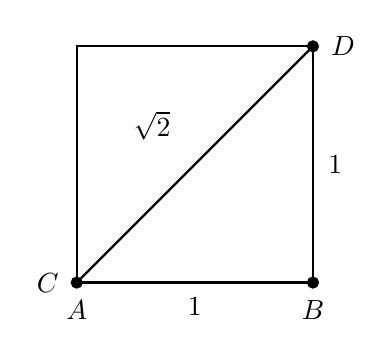
\begin{tikzpicture}[scale=1, >=stealth]
    % Desenho do quadrado e da diagonal (coordenadas multiplicadas por 3)
    \draw[thick] (0,0) -- (3,0) -- (3,3) -- (0,3) -- cycle;
    \draw[thick] (0,0) -- (3,3);

    % Pontos nos vértices A, B, D
    \filldraw[black] (0,0) circle (2pt);
    \filldraw[black] (3,0) circle (2pt);
    \filldraw[black] (3,3) circle (2pt);

    % Rótulos dos vértices
    \node[left=3pt] at (0,0) {$C$};
    \node[below=3pt] at (0,0) {$A$};
    \node[below=3pt] at (3,0) {$B$};
    \node[right=3pt] at (3,3) {$D$};

    % Rótulos dos comprimentos
    \node[below=2pt] at (1.5,0) {$1$};
    \node[right=2pt] at (3,1.5) {$1$};
    \node[above left=1pt] at (1.35,1.65) {$\sqrt{2}$};
  \end{tikzpicture}
  \caption{$\sqrt{2}$ existe como comprimento geométrico.}
  \label{fig:sqrt2-geometria}
\end{figure}

Em vez de abandonar a aritmética em favor da geometria (como os gregos parecem ter feito), nossa solução para essa limitação é fortalecer o conceito de número, passando dos números racionais para um sistema numérico mais amplo. De um ponto de vista moderno, isso deve parecer um fenômeno familiar e bastante natural. Começamos com os \textit{números naturais} \index[remissivo]{números!naturais@\(\mathbb{N}\)}
\[
\mathbb{N} = \{1, 2, 3, 4, 5, \dots\}.
\]

O influente matemático alemão Leopold Kronecker (1823--1891) certa vez afirmou que ``Os números naturais são obra de Deus. Todo o resto é obra do homem''. Discutir a validade dessa afirmação é uma conversa interessante para outro momento. Por ora, ela ao menos nos fornece um ponto de partida. Se restringirmos nossa atenção aos números naturais $\mathbb{N}$, podemos realizar a adição perfeitamente bem, mas precisamos estender nosso sistema para os inteiros \index[remissivo]{números!inteiros@\(\mathbb{Z}\)}
\[
\mathbb{Z} = \{\dots, -3, -2, -1, 0, 1, 2, 3, \dots\}
\]
se quisermos ter uma identidade aditiva (o zero) e os inversos aditivos necessários para definir a subtração. A questão seguinte é a da multiplicação e da divisão. O número $1$ atua como identidade multiplicativa, mas, para definir a divisão, precisamos de inversos multiplicativos. Assim, estendemos nosso sistema novamente para os números racionais \index[remissivo]{números!racionais@\(\mathbb{Q}\)}
\[
\mathbb{Q} = \left\{ \text{todas as frações } \frac{p}{q} \text{, em que } p \text{ e } q \text{ são inteiros com } q \neq 0 \right\}.
\]

Tomadas em conjunto, as propriedades de $\mathbb{Q}$ discutidas no parágrafo 
anterior constituem essencialmente a definição do que se chama em Matemática de um \textit{corpo}.
Enunciado de maneira mais formal, um corpo é um conjunto no qual a adição 
e a multiplicação são operações bem definidas, comutativas, associativas, 
e que obedecem à conhecida propriedade distributiva $a(b + c) = ab + ac$. 
Deve existir uma identidade aditiva, e cada elemento deve possuir um inverso aditivo. 
Por fim, deve existir uma identidade multiplicativa, e inversos 
multiplicativos devem existir para todos os elementos não nulos do corpo. 
Nem $\mathbb{Z}$ nem $\mathbb{N}$ são corpos. O conjunto finito 
$\{0, 1, 2, 3, 4\}$ é um corpo quando a adição e a multiplicação 
são calculadas módulo $5$. Isso não é imediatamente óbvio, 
mas constitui um exercício interessante. \index[remissivo]{corpo}

O conjunto $\mathbb{Q}$ também possui uma ordem natural definida sobre ele. Dados dois números racionais quaisquer $r$ e $s$, vale exatamente uma das alternativas a seguir:
\[
r < s, \quad r = s, \quad \text{ou} \quad r > s.
\]

\begin{figure}[htbp]
  \centering
  \begin{tikzpicture}[scale=0.9, >=stealth]
    % Reta numérica principal
    \draw[thick, ->] (0,0) -- (9.6,0);

    % Pontos pretos preenchidos nos valores de referência (exceto a região de aproximação)
    \foreach \v in {0.8, 0.9, 1.0, 1.1, 1.2, 1.3, 1.5, 1.6, 1.7, 1.8, 1.9, 2.0, 2.1, 2.2} {
      \filldraw[black] ({6*(\v - 0.7)}, 0) circle (2pt);
    }

    % Rótulos dos inteiros e decimais de referência abaixo
    \node[below=5pt] at ({6*(1.0 - 0.7)}, 0) {$1$};
    \node[below=5pt] at ({6*(1.5 - 0.7)}, 0) {$1{,}5$};
    \node[below=5pt] at ({6*(2.0 - 0.7)}, 0) {$2$};

    % Coordenadas separadas para o valor racional aproximante (à esquerda) e a raiz exata (à direita)
    \coordinate (pt1414) at (4.18, 0);
    \coordinate (ptsqrt2) at (4.38, 0);

    % Desenho dos dois pontos distintos na reta
    \filldraw[black] (pt1414) circle (2.2pt);
    \filldraw[red] (ptsqrt2) circle (2.2pt);

    % Indicação de 1,414 (ponto racional aproximante à esquerda)
    \node (bot) at (4.18, -1.55) {$1{,}414$};
    \draw[->, thick] (bot) -- (4.18, -0.15);

    % Indicação de \sqrt{2} (valor real exato à direita)
    \node (top) at (4.38, 1.35) {$\sqrt{2}$};
    \draw[->, thick] (top) -- (4.38, 0.15);
  \end{tikzpicture}
  \caption{Aproximação de $\sqrt{2}$ por números racionais.}
  \label{fig:aproximacao-sqrt2}
\end{figure}

Essa ordenação é transitiva, no sentido de que, se $r < s$ e $s < t$, então $r < t$, o que nos leva convenientemente a uma imagem mental dos números racionais dispostos da esquerda para a direita ao longo de uma reta numérica. Ao contrário do que ocorre com $\mathbb{Z}$, não há intervalos de espaço vazio. Dados dois números racionais quaisquer $r < s$, o número racional $(r+s)/2$ situa-se exatamente no meio entre eles, o que implica que os números racionais estão densamente entrelaçados. \index[remissivo]{densidade} \index[remissivo]{números!racionais@\(\mathbb{Q}\)!densidade} \index[remissivo]{densidade!dos racionais}

Com as propriedades de corpo de $\mathbb{Q}$ permitindo-nos executar com segurança as operações algébricas de adição, subtração, multiplicação e divisão, lembremo-nos daquilo que justamente falta a $\mathbb{Q}$. Pelo \Cref{thm:irracionalidade-sqrt2}, fica evidente que nem sempre podemos extrair raízes quadradas. O problema, no entanto, é na verdade mais fundamental do que isso. Usando apenas números racionais, é possível aproximar $\sqrt{2}$ bastante bem (\Cref{fig:aproximacao-sqrt2}). Por exemplo, $1{,}414^{2} = 1{,}999396$. Acrescentando mais casas decimais à nossa aproximação, podemos nos aproximar ainda mais de um valor para $\sqrt{2}$, mas, ainda assim, estamos agora bem cientes de que há um ``buraco'' na reta numérica racional onde $\sqrt{2}$ deveria estar. É claro que há vários outros buracos --- em $\sqrt{3}$ e $\sqrt{5}$, por exemplo. Retornando ao dilema dos antigos matemáticos gregos, se quisermos que todo comprimento ao longo da reta numérica corresponda a um número de fato, então uma nova extensão do nosso sistema numérico se faz necessária. Assim, à cadeia $\mathbb{N} \subseteq \mathbb{Z} \subseteq \mathbb{Q}$ acrescentamos os números reais $\mathbb{R}$. \index[remissivo]{números!reais@\(\mathbb{R}\)} \index[remissivo]{números!reais@\(\mathbb{R}\)!reta real}

A questão de como efetivamente construir $\mathbb{R}$ a partir de $\mathbb{Q}$ é um assunto bastante complicado. Ela é discutida na \Cref{sec:axioma-completude} e, depois, novamente com mais detalhes na Seção~8.6. Por ora, não é muito impreciso dizer que $\mathbb{R}$ é obtido preenchendo-se as lacunas de $\mathbb{Q}$. Os números reais são, então, a união desses números irracionais com os já familiares números racionais. Que propriedades possui o conjunto dos números irracionais? Como os conjuntos dos números racionais e irracionais se encaixam? Existe uma espécie de simetria entre os racionais e os irracionais, ou há algum sentido em que se possa argumentar que um tipo de número real é mais comum do que o outro? O único método que vimos até agora para gerar exemplos de números irracionais é por meio de raízes quadradas. Não chega a ser surpresa que outras raízes, como $\sqrt[3]{2}$ ou $\sqrt[5]{3}$, sejam na maioria das vezes irracionais. Será que todos os números irracionais podem ser expressos como combinações algébricas de raízes $n$-ésimas e números racionais, ou ainda existem outros números irracionais além daqueles dessa forma? \index[remissivo]{números!irracionais}

% ---------------------------------------------------------------------
% Seção 1.2 — Fundamentos: Conjuntos, Funções e Princípio da Indução
% ---------------------------------------------------------------------

\section{Conjuntos, Funções e o Princípio de Indução}\label{sec:preliminares}

O vocabulário necessário para o desenvolvimento que se segue provém da teoria dos conjuntos e da teoria das funções. Este deve ser um território familiar, mas uma breve revisão da terminologia é provavelmente uma boa ideia, ainda que apenas para estabelecer uma notação acordada.

\subsection{Conjuntos}\label{subsec:conjuntos}

Intuitivamente falando, um \textit{conjunto} é qualquer coleção de objetos. Esses objetos são chamados de \textit{elementos} do conjunto. Para nossos propósitos, os conjuntos em questão serão, na maioria das vezes, conjuntos de números reais, embora também venhamos a encontrar conjuntos de funções e, em algumas ocasiões, conjuntos cujos elementos são outros conjuntos. \index[remissivo]{conjunto} \index[remissivo]{conjunto!elemento}

Dado um conjunto $A$, escrevemos $x \in A$ se $x$ (seja ele o que for) é um elemento de $A$. Se $x$ não é elemento de $A$, escrevemos $x \notin A$. Dados dois conjuntos $A$ e $B$, a \textit{união} é denotada por $A \cup B$ e definida pela regra \index[remissivo]{conjunto!união}
\[
x \in A \cup B \quad \text{desde que} \quad x \in A \text{ ou } x \in B \text{ (possivelmente ambos)}.
\]
A \textit{interseção} $A \cap B$ é o conjunto definido pela regra \index[remissivo]{conjunto!interseção}
\[
x \in A \cap B \quad \text{desde que} \quad x \in A \text{ e } x \in B.
\]

\begin{example}\label{ex:formas-descrever-conjuntos}
\hfill
\begin{enumerate}[label=(\roman*)]
\item Há muitas maneiras aceitáveis de descrever o conteúdo de um conjunto. Na seção anterior, o conjunto dos números naturais foi definido pela listagem de seus elementos: $\mathbb{N} = \{1, 2, 3, \ldots\}$.

\item Conjuntos também podem ser descritos em palavras. Por exemplo, podemos definir o conjunto $E$ como a coleção dos números naturais pares.

\item Algumas vezes é mais eficiente fornecer uma espécie de regra ou algoritmo para determinar os elementos de um conjunto. Como exemplo, seja
\[
S = \{r \in \mathbb{Q} : r^{2} < 2\}.
\]
Lida em voz alta, a definição de $S$ diz: ``Seja $S$ o conjunto de todos os números racionais cujos quadrados são menores que $2$.'' Segue que $1 \in S$, $4/3 \in S$, mas $3/2 \notin S$, pois $9/4 \geq 2$.
\end{enumerate}

Usando os conjuntos definidos acima para ilustrar as operações de interseção e união, observamos que
\[
\mathbb{N} \cup E = \mathbb{N}, \qquad \mathbb{N} \cap E = E, \qquad \mathbb{N} \cap S = \{1\} \qquad \text{e} \qquad E \cap S = \varnothing.
\]
O conjunto $\varnothing$ é chamado de \textit{conjunto vazio} e é entendido como o conjunto que não contém elementos. Uma afirmação equivalente seria dizer que $E$ e $S$ são \textit{disjuntos}.
\end{example}

Uma palavra sobre a igualdade de dois conjuntos é oportuna (já que acabamos de usar essa noção). A relação de \textit{inclusão} $A \subseteq B$, ou $B \supseteq A$, é usada para indicar que todo elemento de $A$ é também elemento de $B$. Nesse caso, dizemos que $A$ é um \textit{subconjunto} de $B$, ou que $B$ \textit{contém} $A$. Afirmar que $A = B$ significa que $A \subseteq B$ e $B \subseteq A$; em outras palavras, $A$ e $B$ possuem exatamente os mesmos elementos. \index[remissivo]{conjunto!subconjunto} \index[remissivo]{conjunto!igualdade}

Com bastante frequência, nos capítulos que virão, vamos querer aplicar as operações de união e interseção a coleções infinitas de conjuntos.

\begin{example}\label{ex:conjuntos-encaixados}
Sejam
\[
\begin{aligned}
A_{1} &= \mathbb{N} = \{1, 2, 3, \dots\}, \\
A_{2} &= \{2, 3, 4, \dots\}, \\
A_{3} &= \{3, 4, 5, \dots\},
\end{aligned}
\]
e, em geral, para cada $n \in \mathbb{N}$, defina o conjunto
\[
A_{n} = \{n, n+1, n+2, \dots\}.
\]
O resultado é uma cadeia encaixada de conjuntos
\[
A_{1} \supseteq A_{2} \supseteq A_{3} \supseteq A_{4} \supseteq \cdots,
\]
na qual cada conjunto sucessivo é subconjunto de todos os anteriores. Em termos de notação,
\[
\bigcup_{n=1}^{\infty} A_{n}, \qquad \bigcup_{n \in \mathbb{N}} A_{n} \qquad \text{ou} \qquad A_{1} \cup A_{2} \cup A_{3} \cup \cdots \index[remissivo]{conjunto!união!infinita}
\]
são todas formas equivalentes de indicar o conjunto formado por todo elemento que aparece em pelo menos um $A_{n}$ específico. Por causa da propriedade de encaixe dessa coleção particular de conjuntos, não é muito difícil ver que
\[
\bigcup_{n=1}^{\infty} A_{n} = A_{1}.
\]
A noção de interseção admite o mesmo tipo de extensão natural para coleções infinitas de conjuntos. Para este exemplo, temos \index[remissivo]{conjunto!interseção!infinita}
\[
\bigcap_{n=1}^{\infty} A_{n} = \varnothing.
\]
Certifiquemo-nos de entender por que esse é o caso. Suponha que houvesse algum número natural $m$ que, a nosso ver, pudesse satisfazer $m \in \bigcap_{n=1}^{\infty} A_{n}$. Isso significaria que $m \in A_{n}$ para \textit{todo} $A_{n}$ de nossa coleção de conjuntos. Como $m$ não é elemento de $A_{m+1}$, tal $m$ não existe, e a interseção é vazia.
\end{example}

Como mencionado, a maioria dos conjuntos que encontraremos será de conjuntos de números reais. Dado $A \subseteq \mathbb{R}$, o \textit{complemento} de $A$, denotado por $A^{c}$, refere-se ao conjunto de todos os elementos de $\mathbb{R}$ que não estão em $A$. Assim, para $A \subseteq \mathbb{R}$, \index[remissivo]{conjunto!complemento}
\[
A^{c} = \{x \in \mathbb{R} : x \notin A\}.
\]

Algumas vezes, em nosso trabalho vindouro, faremos referência às Leis de De Morgan, que afirmam que \index[remissivo]{conjunto!complemento!Leis de De Morgan}
\[
(A \cap B)^{c} = A^{c} \cup B^{c} \qquad \text{e} \qquad (A \cup B)^{c} = A^{c} \cap B^{c}.
\]
As demonstrações dessas afirmações são discutidas no \Cref{ex:de-morgan}.

Há, é preciso admitir, algo de impreciso na definição de conjunto apresentada no início desta discussão. A frase definidora começa com a expressão ``Intuitivamente falando'', o que pode parecer uma maneira estranha de iniciar um curso de estudo que supostamente pretende fornecer uma fundação rigorosa para a teoria das funções de uma variável real. Em certo sentido, porém, isso é inevitável. Cada reparo em um nível da fundação revela algo abaixo dele que necessita de atenção. A teoria dos conjuntos foi submetida a intenso escrutínio ao longo do último século, precisamente porque grande parte da matemática moderna repousa sobre esse fundamento. Mas tal estudo só é realmente aconselhável depois que se entende por que nossa impressão ingênua sobre o comportamento dos conjuntos é insuficiente. Para a direção em que estamos seguindo, isso não acontecerá, embora uma indicação de algumas armadilhas potenciais seja dada na \Cref{sec:epilogo}.

\subsection{Funções}\label{subsec:funcoes}

\index[remissivo]{função} \index[remissivo]{função!domínio} \index[remissivo]{função!imagem}
\begin{definition}\label{def:funcao}
Dados dois conjuntos $A$ e $B$, uma \textit{função} de $A$ em $B$ é uma regra ou aplicação que toma cada elemento $x \in A$ e associa a ele um único elemento de $B$. Nesse caso, escrevemos $f \colon A \to B$. Dado um elemento $x \in A$, a expressão $f(x)$ é usada para representar o elemento de $B$ associado a $x$ por $f$. O conjunto $A$ é chamado de \textit{domínio} de $f$. A \textit{imagem} de $f$ não é necessariamente igual a $B$, mas refere-se ao subconjunto de $B$ dado por $\{y \in B : y = f(x) \text{ para algum } x \in A\}$.
\end{definition}

Essa definição de função é mais ou menos a proposta por Peter Lejeune Dirichlet (1805--1859) na década de 1830. Dirichlet foi um matemático alemão que esteve entre os líderes no desenvolvimento da abordagem rigorosa para funções que estamos prestes a empreender. Sua principal motivação era deslindar as questões que cercam a convergência das séries de Fourier. As contribuições de Dirichlet figuram proeminentemente na Seção~8.5, onde uma introdução às séries de Fourier é apresentada, mas também encontraremos seu nome em vários capítulos anteriores ao longo do caminho. O que é importante no momento é ver como a definição de função de Dirichlet libera o termo de sua interpretação como um tipo de ``fórmula''. Nos anos que antecederam a época de Dirichlet, o termo ``função'' era geralmente entendido como referência a entidades algébricas tais como $f(x) = x^{2} + 1$ ou $g(x) = \sqrt{x^{4} + 4}$. A \Cref{def:funcao} permite uma gama muito mais ampla de possibilidades.

\begin{example}[Função de Dirichlet]\label{ex:funcao-dirichlet}
Em 1829, Dirichlet propôs a exótica função   
\[
g(x) = \begin{cases} 1 & \text{se } x \in \mathbb{Q}, \\ 0 & \text{se } x \notin \mathbb{Q}. \end{cases}
\]
O domínio de $g$ é todo o $\mathbb{R}$, e a imagem é o conjunto $\{0, 1\}$. Não há uma única fórmula para $g$ no sentido usual, e é bastante difícil esboçar o gráfico dessa função (veja a Seção~4.1 para uma tentativa aproximada), mas ela certamente se qualifica como função segundo o critério da \Cref{def:funcao}. À medida que estudarmos a natureza teórica das funções contínuas, diferenciáveis ou integráveis, exemplos como este nos fornecerão um campo de testes inestimável para as muitas conjecturas que encontraremos.
\end{example}

\begin{example}[Desigualdade Triangular]\label{ex:desigualdade-triangular}
A \textit{função valor absoluto} é tão importante que merece a notação especial $|x|$ no lugar do usual $f(x)$ ou $g(x)$. Ela é definida para todo número real por meio da definição por partes \index[remissivo]{função!valor absoluto}
\[
|x| = \begin{cases} x & \text{se } x \geq 0, \\ -x & \text{se } x < 0. \end{cases}
\]
No que diz respeito à multiplicação e à divisão, a função valor absoluto satisfaz
\begin{enumerate}[label=(\roman*)]
\item $|ab| = |a|\,|b|$ e
\item $|a + b| \leq |a| + |b|$
\end{enumerate}
para todas as escolhas de $a$ e $b$. Verificar essas propriedades (\Cref{ex:valor-absoluto-propriedades}) é apenas uma questão de examinar os diferentes casos que surgem quando $a$, $b$ e $a + b$ são positivos e negativos. A propriedade (ii) é chamada de \textit{desigualdade triangular}. Essa desigualdade de aparência inofensiva revela-se fantasticamente importante e será frequentemente empregada da seguinte maneira. Dados três números reais $a$, $b$ e $c$, certamente temos \index[remissivo]{desigualdade triangular}
\[
|a - b| = |(a - c) + (c - b)|.
\]
Pela desigualdade triangular,
\[
|(a - c) + (c - b)| \leq |a - c| + |c - b|,
\]
de modo que obtemos
\[
|a - b| \leq |a - c| + |c - b|. \tag{3}\label{eq:desig-triangular-tres-pontos} \index[remissivo]{desigualdade triangular!três pontos}
\]
Agora, a expressão $|a - b|$ é igual a $|b - a|$ e é mais bem entendida como a \textit{distância} entre os pontos $a$ e $b$ na reta numérica. Com essa interpretação, a equação~\eqref{eq:desig-triangular-tres-pontos} faz a afirmação plausível de que a distância de $a$ até $b$ é menor ou igual à distância de $a$ até $c$ mais a distância de $c$ até $b$. Fingindo por um momento que esses são pontos no plano (em vez de pontos na reta real), deve ficar evidente por que isso é chamado de ``desigualdade triangular''.
\end{example}

\subsection{Lógica e Demonstrações}\label{subsec:logica-demonstracoes}

Escrever demonstrações matemáticas rigorosas é uma habilidade que se aprende melhor praticando, e haverá muito treinamento em serviço logo à frente. Como Hardy indica, há uma qualidade artística na matemática desse tipo, que pode ou não vir com facilidade, mas isso não quer dizer que algo de especialmente misterioso esteja acontecendo. Uma demonstração é uma espécie de ensaio. É um conjunto de instruções cuidadosamente elaboradas que, quando seguidas, devem deixar o leitor absolutamente convencido da verdade da proposição em questão. Para alcançar isso, os passos de uma demonstração devem decorrer logicamente de passos anteriores ou ser justificados por algum outro conjunto de fatos acordado. Além de válidos, esses passos devem também se encaixar coerentemente para formar um argumento convincente. A matemática tem um vocabulário especializado, sem dúvida, mas isso não exime uma boa demonstração de ser escrita em português gramaticalmente correto.

A única demonstração que vimos até este ponto (a do \Cref{thm:irracionalidade-sqrt2}) usa uma estratégia indireta chamada \textit{demonstração por contradição}. Essa técnica poderosa será empregada diversas vezes em nosso trabalho vindouro. Não obstante, a maioria das demonstrações é direta. (Vale também mencionar que usar uma demonstração indireta quando uma demonstração direta está disponível é geralmente considerado de mau tom.) Uma demonstração direta começa a partir de alguma afirmação válida, mais frequentemente tomada da hipótese do teorema, e então prossegue por deduções rigorosamente lógicas até estabelecer a conclusão do teorema. Como vimos no \Cref{thm:irracionalidade-sqrt2}, uma demonstração indireta sempre começa negando aquilo que gostaríamos de provar. Isso nem sempre é tão fácil de fazer quanto pode parecer. O argumento então prossegue até que (esperançosamente) uma contradição lógica com algum outro fato aceito seja descoberta. Muitas vezes, esse fato aceito é parte da hipótese do teorema. Quando a contradição é com a hipótese do teorema, temos tecnicamente o que se chama de \textit{demonstração por contraposição}. \index[remissivo]{demonstração!por contraposição}

A próxima proposição ilustra diversas das questões recém-discutidas e introduz algumas outras.

\begin{theorem}\label{thm:epsilon-igualdade}
Dois números reais $a$ e $b$ são iguais se, e somente se, para todo número real $\epsilon > 0$, vale $|a - b| < \epsilon$.
\end{theorem}

\begin{proof}
Há duas frases-chave no enunciado desta proposição que merecem atenção especial. Uma é ``para todo'', que será tratada daqui a pouco. A outra é ``se, e somente se''. Dizer ``se, e somente se'' em matemática é uma maneira econômica de afirmar que a proposição é verdadeira em duas direções. Na direção direta, devemos provar a afirmação: \index[remissivo]{quantificador}
\[
(\Rightarrow) \quad \text{Se } a = b, \text{ então, para todo número real } \epsilon > 0, \text{ vale } |a - b| < \epsilon.
\]
Devemos também provar a afirmação recíproca:
\[
(\Leftarrow) \quad \text{Se, para todo número real } \epsilon > 0, \text{ vale } |a - b| < \epsilon, \text{ então devemos ter } a = b.
\]
Para a demonstração da primeira afirmação, não há realmente muito o que dizer. Se $a = b$, então $|a - b| = 0$ e, portanto, certamente $|a - b| < \epsilon$, não importa qual $\epsilon > 0$ seja escolhido.

Para a segunda afirmação, damos uma demonstração por contradição. A conclusão da proposição nesta direção afirma que $a = b$, de modo que supomos $a \neq b$. Partindo em busca de uma contradição, somos levados a considerar a frase ``para todo $\epsilon > 0$''. Algumas maneiras equivalentes de enunciar a hipótese seriam dizer que ``para toda escolha possível de $\epsilon > 0$'' ou ``não importa como $\epsilon > 0$ seja selecionado, é sempre verdade que $|a - b| < \epsilon$''. Mas, supondo $a \neq b$ (como estamos fazendo neste momento), a escolha de
\[
\epsilon_{0} = |a - b| > 0
\]
coloca um sério problema. Estamos supondo que $|a - b| < \epsilon$ é verdadeiro para todo $\epsilon > 0$, de modo que isso certamente deve ser verdadeiro para o $\epsilon_{0}$ particular recém-definido. No entanto, as afirmações
\[
|a - b| < \epsilon_{0} \qquad \text{e} \qquad |a - b| = \epsilon_{0}
\]
não podem ser ambas verdadeiras. Essa contradição significa que nossa suposição inicial de que $a \neq b$ é inaceitável. Portanto, $a = b$, e a demonstração indireta está completa.
\end{proof}

Uma das habilidades mais fundamentais exigidas para ler e escrever demonstrações em Análise Real é a capacidade de manipular com confiança as frases quantificadoras ``para todo'' e ``existe''. Significativamente mais atenção será dada a essa questão em muitas discussões vindouras.

\subsection{Indução}\label{subsec:inducao}

Uma última ferramenta fundamental, que surgirá com certa frequência, é o uso de argumentos por \textit{indução}. A indução é usada em conjunto com os números naturais $\mathbb{N}$ (ou, algumas vezes, com o conjunto $\mathbb{N} \cup \{0\}$). O princípio fundamental por trás da indução é que, se $S$ é algum subconjunto de $\mathbb{N}$ com a propriedade de que \index[remissivo]{indução matemática} \index[remissivo]{números!naturais@\(\mathbb{N}\)!indução}
\begin{enumerate}[label=(\roman*)]
\item $S$ contém o número $1$, e
\item sempre que $S$ contém um número natural $n$, contém também $n + 1$,
\end{enumerate}
então deve ser $S = \mathbb{N}$. Como o próximo exemplo ilustra, esse princípio pode ser usado tanto para definir sequências de objetos quanto para provar fatos sobre elas.

\begin{example}\label{ex:inducao-sequencia}
Seja $x_{1} = 1$ e, para cada $n \in \mathbb{N}$, defina
\[
x_{n+1} = \frac{1}{2}\, x_{n} + 1.
\]
Usando essa regra, podemos calcular $x_{2} = (1/2)(1) + 1 = 3/2$, $x_{3} = 7/4$, e é imediatamente aparente como isso conduz a uma definição de $x_{n}$ para todo $n \in \mathbb{N}$. \index[remissivo]{sequência}

A sequência recém-definida parece, à primeira vista, ser crescente. Para os termos calculados, temos $x_{1} \leq x_{2} \leq x_{3}$. Usemos a indução para provar que essa tendência continua; isto é, mostremos que \index[remissivo]{sequência!monótona} \index[remissivo]{sequência!monótona!crescente}
\[
x_{n} \leq x_{n+1} \tag{4}\label{eq:inducao-afirmacao}
\]
para todo $n \in \mathbb{N}$.

Para $n = 1$, $x_{1} = 1$ e $x_{2} = 3/2$, de modo que $x_{1} \leq x_{2}$ é claro. Agora, queremos mostrar que
\[
\text{se temos } x_{n} \leq x_{n+1}, \text{ então segue que } x_{n+1} \leq x_{n+2}.
\]
Pense em $S$ como o conjunto dos números naturais para os quais a afirmação da equação~\eqref{eq:inducao-afirmacao} é verdadeira. Mostramos que $1 \in S$. Estamos agora interessados em mostrar que, se $n \in S$, então $n + 1 \in S$ também. Partindo da hipótese de indução $x_{n} \leq x_{n+1}$, podemos multiplicar a desigualdade por $1/2$ e somar $1$ a ambos os lados para obter
\[
\frac{1}{2}\, x_{n} + 1 \leq \frac{1}{2}\, x_{n+1} + 1,
\]
que é precisamente a conclusão desejada $x_{n+1} \leq x_{n+2}$. Por indução, a afirmação está provada para todo $n \in \mathbb{N}$.
\end{example}

Qualquer discussão sobre por que a indução é uma técnica argumentativa válida abre imediatamente uma caixa de questões sobre como entendemos os números naturais. Antes, na \Cref{sec:irracionalidade-sqrt2}, evitamos essa questão recorrendo ao famoso comentário de Kronecker de que os números naturais são, de alguma forma, dados divinamente. Embora não pretendamos aprimorar essa explicação aqui, deve-se assinalar que uma abordagem mais ateísta e matematicamente satisfatória para $\mathbb{N}$ é possível do ponto de vista da teoria axiomática dos conjuntos. Isso nos traz de volta a um tema recorrente deste capítulo. Pedagogicamente falando, os fundamentos da matemática são mais bem aprendidos e apreciados em uma espécie de ordem inversa. Um estudo rigoroso dos números naturais e da teoria dos conjuntos é certamente recomendado, mas somente depois que tivermos compreensão das sutilezas do sistema dos números reais. É este último tópico o verdadeiro negócio da análise real.

\subsection{Lista de Exercícios}\label{subsec:exercicios-preliminares}

\begin{exercise}\label{ex:raiz3-irracional}
\begin{enumerate}[label=\alph*)]
\item Prove que $\sqrt{3}$ é irracional. Um argumento semelhante funciona para mostrar que $\sqrt{6}$ é irracional?
\item Onde a demonstração do \Cref{thm:irracionalidade-sqrt2} falha se tentarmos usá-la para provar que $\sqrt{4}$ é irracional?
\end{enumerate}
\end{exercise}

\begin{exercise}\label{ex:potencia-racional}
Mostre que não existe número racional $r$ satisfazendo $2^{r} = 3$.
\end{exercise}

\begin{exercise}\label{ex:verdadeiro-falso-conjuntos}
Decida quais das afirmações a seguir são verdadeiras sobre a natureza dos conjuntos. Para as que forem falsas, forneça um exemplo específico em que a afirmação em questão não vale.
\begin{enumerate}[label=\alph*)]
\item Se $A_{1} \supseteq A_{2} \supseteq A_{3} \supseteq A_{4} \supseteq \cdots$ são todos conjuntos contendo um número infinito de elementos, então a interseção $\bigcap_{n=1}^{\infty} A_{n}$ é também infinita.
\item Se $A_{1} \supseteq A_{2} \supseteq A_{3} \supseteq A_{4} \supseteq \cdots$ são todos conjuntos finitos, não vazios, de números reais, então a interseção $\bigcap_{n=1}^{\infty} A_{n}$ é finita e não vazia.
\item $A \cap (B \cup C) = (A \cap B) \cup C$.
\item $A \cap (B \cap C) = (A \cap B) \cap C$.
\item $A \cap (B \cup C) = (A \cap B) \cup (A \cap C)$.
\end{enumerate}
\end{exercise}

\begin{exercise}\label{ex:particao-infinita-de-N}
Produza uma coleção infinita de conjuntos $A_{1}, A_{2}, A_{3}, \ldots$ com a propriedade de que cada $A_{i}$ tem um número infinito de elementos, $A_{i} \cap A_{j} = \varnothing$ para todos $i \neq j$, e $\bigcup_{i=1}^{\infty} A_{i} = \mathbb{N}$.
\end{exercise}

\begin{exercise}[Leis de De Morgan]\label{ex:de-morgan}
Sejam $A$ e $B$ subconjuntos de $\mathbb{R}$.
\begin{enumerate}[label=\alph*)]
\item Se $x \in (A \cap B)^{c}$, explique por que $x \in A^{c} \cup B^{c}$. Isso mostra que $(A \cap B)^{c} \subseteq A^{c} \cup B^{c}$.
\item Prove a inclusão reversa $(A \cap B)^{c} \supseteq A^{c} \cup B^{c}$ e conclua que $(A \cap B)^{c} = A^{c} \cup B^{c}$.
\item Mostre que $(A \cup B)^{c} = A^{c} \cap B^{c}$ demonstrando a inclusão em ambas as direções.
\end{enumerate}
\end{exercise}

\begin{exercise}\label{ex:valor-absoluto-propriedades}
\begin{enumerate}[label=\alph*)]
\item Verifique a desigualdade triangular no caso especial em que $a$ e $b$ têm o mesmo sinal.
\item Encontre uma demonstração eficiente para todos os casos de uma só vez, demonstrando primeiro que $(a + b)^{2} \leq (|a| + |b|)^{2}$.
\item Prove que $|a - b| \leq |a - c| + |c - d| + |d - b|$ para todos $a$, $b$, $c$ e $d$.
\item Prove que $\bigl||a| - |b|\bigr| \leq |a - b|$. (A identidade pouco notável $a = a - b + b$ pode ser útil.)
\end{enumerate}
\end{exercise}

\begin{exercise}\label{ex:imagem-de-conjuntos}
Dada uma função $f$ e um subconjunto $A$ de seu domínio, seja $f(A)$ a imagem de $f$ sobre o conjunto $A$; isto é, $f(A) = \{f(x) : x \in A\}$.
\begin{enumerate}[label=\alph*)]
\item Seja $f(x) = x^{2}$. Se $A = [0, 2]$ (o intervalo fechado $\{x \in \mathbb{R} : 0 \leq x \leq 2\}$) e $B = [1, 4]$, encontre $f(A)$ e $f(B)$. Neste caso, vale $f(A \cap B) = f(A) \cap f(B)$? Vale $f(A \cup B) = f(A) \cup f(B)$? \index[remissivo]{intervalo} \index[remissivo]{intervalo!fechado}
\item Encontre dois conjuntos $A$ e $B$ para os quais $f(A \cap B) \neq f(A) \cap f(B)$.
\item Mostre que, para uma função arbitrária $g \colon \mathbb{R} \to \mathbb{R}$, é sempre verdade que $g(A \cap B) \subseteq g(A) \cap g(B)$ para todos os conjuntos $A, B \subseteq \mathbb{R}$.
\item Formule e prove uma conjectura sobre a relação entre $g(A \cup B)$ e $g(A) \cup g(B)$ para uma função arbitrária $g$.
\end{enumerate}
\end{exercise}

\begin{exercise}\label{ex:injetora-sobrejetora}
Eis duas definições importantes relativas a uma função $f \colon A \to B$. A função $f$ é \textit{injetora} se $a_{1} \neq a_{2}$ em $A$ implica $f(a_{1}) \neq f(a_{2})$ em $B$. A função $f$ é \textit{sobrejetora} se, dado qualquer $b \in B$, é possível encontrar um elemento $a \in A$ para o qual $f(a) = b$. \index[remissivo]{função!injetora} \index[remissivo]{função!sobrejetora}

Dê um exemplo de cada uma das situações a seguir ou declare que o pedido é impossível:
\begin{enumerate}[label=\alph*)]
\item $f \colon \mathbb{N} \to \mathbb{N}$ que seja injetora, mas não sobrejetora.
\item $f \colon \mathbb{N} \to \mathbb{N}$ que seja sobrejetora, mas não injetora.
\item $f \colon \mathbb{N} \to \mathbb{Z}$ que seja injetora e sobrejetora.
\end{enumerate}
\end{exercise}

\begin{exercise}\label{ex:pre-imagem}
Dada uma função $f \colon D \to \mathbb{R}$ e um subconjunto $B \subseteq \mathbb{R}$, seja $f^{-1}(B)$ o conjunto de todos os pontos do domínio $D$ que são mapeados em $B$; isto é, 
$$f^{-1}(B) = \{x \in D : f(x) \in B\}.$$ 
Esse conjunto é chamado de \textit{pré-imagem} (ou imagem inversa) de $B$. \index[remissivo]{pre@pré-imagem}
\begin{enumerate}[label=\alph*)]
\item Seja $f(x) = x^{2}$. Se $A$ é o intervalo fechado $[0, 4]$ e $B$ é o intervalo fechado $[-1, 1]$, encontre $f^{-1}(A)$ e $f^{-1}(B)$. Neste caso, vale $f^{-1}(A \cap B) = f^{-1}(A) \cap f^{-1}(B)$? Vale $f^{-1}(A \cup B) = f^{-1}(A) \cup f^{-1}(B)$?
\item O bom comportamento das pré-imagens demonstrado no item (a) é completamente geral. Mostre que, para uma função arbitrária $g \colon \mathbb{R} \to \mathbb{R}$, é sempre verdade que $g^{-1}(A \cap B) = g^{-1}(A) \cap g^{-1}(B)$ e $g^{-1}(A \cup B) = g^{-1}(A) \cup g^{-1}(B)$ para todos os conjuntos $A, B \subseteq \mathbb{R}$.
\end{enumerate}
\end{exercise}

\begin{exercise}\label{ex:epsilon-desigualdades}
Decida quais das afirmações a seguir são verdadeiras. Forneça uma justificativa curta para as que forem válidas e um contraexemplo para as que não forem:
\begin{enumerate}[label=\alph*)]
\item Dois números reais satisfazem $a < b$ se, e somente se, $a < b + \epsilon$ para todo $\epsilon > 0$.
\item Dois números reais satisfazem $a < b$ se $a < b + \epsilon$ para todo $\epsilon > 0$.
\item Dois números reais satisfazem $a \leq b$ se, e somente se, $a < b + \epsilon$ para todo $\epsilon > 0$.
\end{enumerate}
\end{exercise}

\begin{exercise}\label{ex:negacao-logica}
Formule a negação lógica de cada uma das afirmações abaixo. 
Para tornar este exercicio mais interessante, 
formule a negação como uma afirmação e evite completamente o uso da palavra ``não''. 
Em cada caso, dê seu palpite intuitivo sobre a validade da afirmação original ou de sua negação.
\begin{enumerate}[label=\alph*)]
\item Para todos os números reais satisfazendo $a < b$, existe um $n \in \mathbb{N}$ tal que $a + 1/n < b$.
\item Existe um número real $x > 0$ tal que $x < 1/n$ para todo $n \in \mathbb{N}$.
\item Entre quaisquer dois números reais distintos há um número racional.
\end{enumerate}
\end{exercise}

\begin{exercise}\label{ex:inducao-sequencia-y}
Seja $y_{1} = 6$ e, para cada $n \in \mathbb{N}$, defina $y_{n+1} = (2 y_{n} - 6)/3$.
\begin{enumerate}[label=\alph*)]
\item Use indução para provar que a sequência satisfaz $y_{n} > -6$ para todo $n \in \mathbb{N}$.
\item Use outro argumento por indução para mostrar que a sequência $(y_{1}, y_{2}, y_{3}, \ldots)$ é decrescente.
\end{enumerate}
\end{exercise}

\begin{exercise}\label{ex:de-morgan-inducao}
Para este exercício, suponha que o \Cref{ex:de-morgan} tenha sido completado com sucesso.
\begin{enumerate}[label=\alph*)]
\item Mostre como a indução pode ser usada para concluir que
\[
(A_{1} \cup A_{2} \cup \cdots \cup A_{n})^{c} = A_{1}^{c} \cap A_{2}^{c} \cap \cdots \cap A_{n}^{c}
\]
para qualquer $n \in \mathbb{N}$ finito.
\item É tentador apelar à indução para concluir que
\[
\left( \bigcup_{i=1}^{\infty} A_{i} \right)^{c} = \bigcap_{i=1}^{\infty} A_{i}^{c},
\]
mas a indução não se aplica aqui. A indução é usada para provar que uma afirmação particular vale para todo $n \in \mathbb{N}$, mas isso não implica a validade do caso infinito. Para ilustrar esse ponto, encontre um exemplo de uma coleção de conjuntos $B_{1}, B_{2}, B_{3}, \ldots$ em que $\bigcap_{i=1}^{n} B_{i} \neq \varnothing$ é verdadeiro para todo $n \in \mathbb{N}$, mas $\bigcap_{i=1}^{\infty} B_{i} \neq \varnothing$ falha.
\end{enumerate}
\end{exercise}

% ---------------------------------------------------------------------
% Seção 1.3 — O Axioma da Completude
% ---------------------------------------------------------------------

\index[remissivo]{Axioma da Completude}
\section{O Axioma da Completude}\label{sec:axioma-completude}

O que exatamente é um número real? Na \Cref{sec:irracionalidade-sqrt2}, chegamos ao ponto de dizer que o conjunto $\mathbb{R}$ dos números reais é uma extensão do conjunto dos números racionais $\mathbb{Q}$ na qual não há buracos ou lacunas. Queremos que todo comprimento ao longo da reta numérica --- como $\sqrt{2}$, por exemplo --- corresponda a um número real, e vice-versa. \index[remissivo]{números!reais@\(\mathbb{R}\)!reta real}

Vamos aprimorar essa definição, mas, ao fazê-lo, é importante ter em mente nossa observação anterior de que quaisquer enunciados precisos que formulemos repousarão necessariamente sobre outras hipóteses não demonstradas ou termos indefinidos. Em algum momento, precisamos traçar uma linha e confessar que é isso que decidimos aceitar como um ponto de partida razoável. Naturalmente, há certo debate sobre onde essa linha deve ser traçada. Uma maneira de ver a matemática dos séculos XIX e XX é encará-la como uma tentativa obstinada de empurrar essa linha cada vez mais para trás, em direção a alguma fundação inabalável. A maior parte do material coberto nesta notas é atribuível aos matemáticos que trabalharam no início e em meados do século XIX. Augustin Louis Cauchy (1789--1857), Bernhard Bolzano (1781--1848), Niels Henrik Abel (1802--1829), Peter Lejeune Dirichlet, Karl Weierstrass (1815--1897) e Bernhard Riemann (1826--1866) figuraram de maneira proeminente na descoberta dos teoremas que se seguem. Mas eis o ponto interessante. Quase todo esse trabalho foi feito usando hipóteses intuitivas sobre a natureza de $\mathbb{R}$ bastante semelhantes à nossa própria compreensão informal neste momento. Eventualmente, escrutínio suficiente foi dirigido à estrutura detalhada de $\mathbb{R}$, de modo que, na década de 1870, algumas poucas maneiras de construir $\mathbb{R}$ rigorosamente a partir de $\mathbb{Q}$ foram propostas.

A construção rigorosa de $\mathbb{R}$ a partir de $\mathbb{Q}$, seguindo esse modelo histórico, 
é apresentada na Seção~8.6 da referência \cite{MR3331079}. 


\subsection{Uma Definição Inicial para $\mathbb{R}$}\label{subsec:definicao-inicial-R}

Primeiro, $\mathbb{R}$ é um conjunto que contém $\mathbb{Q}$. As operações de adição e multiplicação em $\mathbb{Q}$ estendem-se a todo $\mathbb{R}$ de tal maneira que todo elemento de $\mathbb{R}$ possui um inverso aditivo e todo elemento não nulo de $\mathbb{R}$ possui um inverso multiplicativo. Ecoando a discussão da \Cref{sec:irracionalidade-sqrt2}, supomos que $\mathbb{R}$ é um \textit{corpo}, o que significa que a adição e a multiplicação de números reais são comutativas e associativas, e a propriedade distributiva é válida. Isso nos permite realizar todas as manipulações algébricas padrões que fazem parte do nosso cotidiano. Supomos também que as propriedades familiares da ordenação em $\mathbb{Q}$ se estendem a todo $\mathbb{R}$. Assim, por exemplo, deduções como ``Se $a < b$ e $c > 0$, então $ac < bc$'' serão realizadas livremente, sem muitos comentários. Para resumir a situação na terminologia oficial da área, supomos que $\mathbb{R}$ é um \textit{corpo ordenado}, que contém $\mathbb{Q}$ como subcorpo. (Uma definição rigorosa de ``corpo ordenado'' 
pode ser vista na Seção~8.6 de \cite{MR3331079}) \index[remissivo]{números!reais@\(\mathbb{R}\)} \index[remissivo]{corpo!ordenado}

Isso nos traz à última, e mais distintiva, hipótese sobre o sistema dos números reais. Precisamos encontrar alguma maneira de articular claramente o que queremos dizer ao insistir que $\mathbb{R}$ não contém as lacunas que permeiam $\mathbb{Q}$. Como essa é a diferença definidora entre os números racionais e os números reais, seremos excessivamente precisos quanto à maneira de enunciar essa hipótese, doravante chamada de \textit{Axioma da Completude}. \index[remissivo]{corpo!ordenado!completude}

\bigskip 

\index[remissivo]{Axioma da Completude!menor cota superior} \index[remissivo]{supremo!existência}
\noindent\textbf{Axioma da Completude.} \textit{Todo conjunto não vazio de números reais que é limitado superiormente possui uma menor cota superior.}


\bigskip 


Agora, o que exatamente isso significa?

\subsection{Menores Cotas Superiores e Maiores Cotas Inferiores}\label{subsec:menores-cotas}

Vamos primeiro enunciar as definições relevantes e, em seguida, examinar alguns exemplos.

\begin{definition}\label{def:cotas-superiores-inferiores}
Um conjunto $A \subseteq \mathbb{R}$ é \textit{limitado superiormente} se existe um número $b \in \mathbb{R}$ tal que $a \leq b$ para todo $a \in A$. O número $b$ é chamado de \textit{cota superior} de $A$. \index[remissivo]{cota!superior} \index[remissivo]{cota!superior!conjunto limitado superiormente} \index[remissivo]{conjunto!limitado}

De modo semelhante, o conjunto $A$ é \textit{limitado inferiormente} se existe uma \textit{cota inferior} $l \in \mathbb{R}$ satisfazendo $l \leq a$ para todo $a \in A$. \index[remissivo]{cota!inferior} \index[remissivo]{cota!inferior!conjunto limitado inferiormente}
\end{definition}

\break 


\begin{definition}\label{def:menor-cota-superior}
Um número real $s$ é a \textit{menor cota superior} (ou \textit{cota superior mínima}) de um conjunto $A \subseteq \mathbb{R}$ se satisfaz os dois critérios a seguir: \index[remissivo]{supremo} \index[remissivo]{supremo!definição}
\begin{enumerate}[label=(\roman*)]
\item $s$ é uma cota superior de $A$;
\item se $b$ é qualquer cota superior de $A$, então $s \leq b$.
\end{enumerate}
\end{definition}

A menor cota superior é também frequentemente chamada de \textit{supremo} do conjunto $A$,
notação $\sup A$. Por outro lado, a \textit{maior cota inferior} ou \textit{ínfimo} de $A$ é definida de modo semelhante (veja o \Cref{ex:definicao-infimo}) e é denotada por $\inf A$ (\Cref{fig:def-sup-inf}). \index[remissivo]{infimo@ínfimo} \index[remissivo]{infimo@ínfimo!definição}

\begin{figure}[htbp]
  \centering
  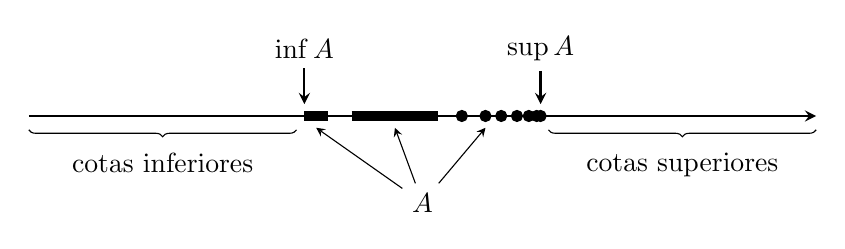
\begin{tikzpicture}[scale=1.0, >=stealth]
    % Reta real principal
    \draw[thick, ->] (0,0) -- (10,0);

    % Primeira barra sólida à esquerda de A
    \draw[line width=3.5pt] (3.5,0) -- (3.8,0);

    % Segunda barra sólida de A separada da primeira por um pequeno espaço
    \draw[line width=3.5pt] (4.1,0) -- (5.2,0);

    % Pontos discretos do conjunto A acumulando-se à direita
    \foreach \x in {5.5, 5.8, 6.0, 6.2, 6.35, 6.45, 6.5} {
      \filldraw[black] (\x,0) circle (2pt);
    }

    % Chaves inferiores para cotas inferiores e cotas superiores
    \draw [decorate, decoration={brace, mirror, raise=5pt}] (0,0) -- (3.4,0)
      node[pos=0.5, below=10pt] {cotas inferiores};

    \draw [decorate, decoration={brace, mirror, raise=5pt}] (6.6,0) -- (10,0)
      node[pos=0.5, below=10pt] {cotas superiores};

    % Indicação do conjunto A com 3 setas apontando para cada uma das partes de A
    \node (A) at (5.0, -1.1) {$A$};
    \draw[->] (A) -- (3.65, -0.15);
    \draw[->] (A) -- (4.65, -0.15);
    \draw[->] (A) -- (5.8, -0.15);

    % Indicação de inf A
    \node (inf) at (3.5, 0.85) {$\inf A$};
    \draw[->, thick] (inf) -- (3.5, 0.15);

    % Indicação de sup A
    \node (sup) at (6.5, 0.85) {$\sup A$};
    \draw[->, thick] (sup) -- (6.5, 0.15);
  \end{tikzpicture}
  \caption{Definição de $\sup A$ e $\inf A$.}
  \label{fig:def-sup-inf}
\end{figure}

Embora um conjunto possa ter uma infinidade de cotas superiores, ele pode ter apenas uma \textit{menor} cota superior. Se $s_{1}$ e $s_{2}$ são ambas menores cotas superiores de um conjunto $A$, então, pela propriedade (ii) da \Cref{def:menor-cota-superior}, podemos afirmar $s_{1} \leq s_{2}$ e $s_{2} \leq s_{1}$. A conclusão é que $s_{1} = s_{2}$, e as menores cotas superiores são únicas.

\begin{example}\label{ex:sup-de-1n}
Seja
\[
A = \left\{ \frac{1}{n} : n \in \mathbb{N} \right\} = \left\{ 1, \frac{1}{2}, \frac{1}{3}, \dots \right\}.
\]
O conjunto $A$ é limitado superiormente e inferiormente. Candidatos bem-sucedidos a cota superior incluem $3$, $2$ e $3/2$. Para a menor cota superior, afirmamos que $\sup A = 1$. Para argumentar isso rigorosamente usando a \Cref{def:menor-cota-superior}, precisamos verificar que as propriedades (i) e (ii) valem. Para (i), basta observar que $1 \geq 1/n$ para todas as escolhas de $n \in \mathbb{N}$. Para verificar (ii), começamos supondo que temos alguma outra cota superior $b$. Como $1 \in A$ e $b$ é uma cota superior de $A$, devemos ter $1 \leq b$. Isso é precisamente o que a propriedade (ii) nos pede para mostrar.

Embora ainda não tenhamos exatamente as ferramentas necessárias para uma demonstração rigorosa (veja a \Cref{thm:propriedade-arquimediana}), deve ser razoavelmente aparente que $\inf A = 0$.
\end{example}

Uma lição importante a extrair do \Cref{ex:sup-de-1n} é que $\sup A$ e $\inf A$ podem ou não ser elementos do conjunto $A$. Essa questão está ligada à compreensão da diferença crucial entre o máximo e o supremo (ou o mínimo e o ínfimo) de um dado conjunto.

\begin{definition}\label{def:maximo-minimo}
Um número real $a_{0}$ é um \textit{máximo} do conjunto $A$ se $a_{0}$ é um elemento de $A$ e $a_{0} \geq a$ para todo $a \in A$. De modo semelhante, um número $a_{1}$ é um \textit{mínimo} de $A$ se $a_{1} \in A$ e $a_{1} \leq a$ para todo $a \in A$. \index[remissivo]{máximo} \index[remissivo]{mínimo} \index[remissivo]{mínimo!versus ínfimo}
\end{definition}

\begin{example}\label{ex:maximo-vs-supremo}
Para insistir no ponto, considere o intervalo aberto \index[remissivo]{intervalo} \index[remissivo]{intervalo!aberto}
\[
(0, 2) = \{ x \in \mathbb{R} : 0 < x < 2 \},
\]
e o intervalo fechado \index[remissivo]{intervalo!fechado}
\[
[0, 2] = \{ x \in \mathbb{R} : 0 \leq x \leq 2 \}.
\]
Ambos os conjuntos são limitados superiormente (e inferiormente), e ambos têm a mesma menor cota superior, a saber, $2$. No entanto, \textit{não} é o caso que ambos os conjuntos tenham um máximo. Um máximo é um tipo específico de cota superior que precisa ser um elemento do conjunto em questão, e o intervalo aberto $(0, 2)$ não possui tal elemento. Assim, o supremo pode existir e não ser um máximo, mas, quando um máximo existe, ele é também o supremo. \index[remissivo]{máximo!versus supremo}
\end{example}

Voltemos nossa atenção ao Axioma da Completude. Embora possamos ver agora que nem todo conjunto não vazio e limitado contém um máximo, o Axioma da Completude afirma que todo conjunto desse tipo possui de fato uma menor cota superior. Não vamos demonstrar isso. Um \textit{axioma} em matemática é uma hipótese aceita, a ser usada sem demonstração. Preferencialmente, um axioma deve ser um enunciado elementar sobre o sistema em questão, tão fundamental que parece não necessitar de justificação. Talvez o Axioma da Completude se encaixe nessa descrição, talvez não. Antes de decidir, lembremo-nos de por que \textit{ele não é um enunciado válido sobre} $\mathbb{Q}$.

\begin{example}\label{ex:conjunto-r2-menor-2}
Considere novamente o conjunto
\[
S = \{ r \in \mathbb{Q} : r^{2} < 2 \},
\]
e finja por um momento que nosso mundo é constituído apenas de números racionais. O conjunto $S$ é certamente limitado superiormente. Tomar $b = 2$ funciona, assim como $b = 3/2$. Mas observe o que acontece quando partimos em busca da \textit{menor} cota superior. (Pode ser útil saber aqui que a expansão decimal de $\sqrt{2}$ começa com $1{,}4142\ldots$.) Podemos tentar $b = 142/100$, que é de fato uma cota superior, mas então descobrimos que $b = 1415/1000$ é uma cota superior ainda menor. Existe uma menor de todas?

Nos números racionais, não existe. Nos números reais, existe. De volta em $\mathbb{R}$, o Axioma da Completude afirma que podemos tomar $\alpha = \sup S$ e estar confiantes de que tal número existe. Na próxima seção, provaremos que $\alpha^{2} = 2$. Mas, de acordo com o \Cref{thm:irracionalidade-sqrt2}, isso implica que $\alpha$ não é um número racional. Se estamos restringindo nossa atenção apenas aos números racionais, então $\alpha$ não é uma opção permitida para $\sup S$, e a busca por uma menor cota superior continua indefinidamente. Qualquer que seja a cota superior racional descoberta, é sempre possível encontrar uma menor.
\end{example}

As ferramentas necessárias para realizar os cálculos descritos no \Cref{ex:conjunto-r2-menor-2} dependem de resultados sobre como $\mathbb{Q}$ e $\mathbb{N}$ se encaixam dentro de $\mathbb{R}$. Esses resultados são discutidos na próxima seção. Nesse meio tempo, é possível provar algumas propriedades algébricas intuitivas das menores cotas superiores usando apenas a definição.

\begin{example}\label{ex:sup-translacao}
Seja $A \subseteq \mathbb{R}$ não vazio e limitado superiormente, e seja $c \in \mathbb{R}$. Defina o conjunto $c + A$ por
\[
c + A \equiv  \{ c + a : a \in A \}.
\]
Então, 
$$\sup(c + A) = c + \sup A.$$

Para verificar isso adequadamente, enfocamos separadamente cada parte da \Cref{def:menor-cota-superior}. Tomando $s = \sup A$, vemos que $a \leq s$ para todo $a \in A$, o que implica $c + a \leq c + s$ para todo $a \in A$. Assim, $c + s$ é uma cota superior de $c + A$, e a condição (i) está verificada.

Para (ii), seja $b$ uma cota superior arbitrária de $c + A$; isto é, $c + a \leq b$ para todo $a \in A$. Isso é equivalente a $a \leq b - c$ para todo $a \in A$, de onde concluímos que $b - c$ é uma cota superior de $A$. Como $s$ é a \textit{menor} cota superior de $A$, temos $s \leq b - c$, o que pode ser reescrito como $c + s \leq b$. Isso verifica a parte (ii) da \Cref{def:menor-cota-superior}, e concluímos que $\sup(c + A) = c + \sup A$.
\end{example}

Há uma maneira equivalente e útil de caracterizar as menores cotas superiores. Como o exemplo anterior ilustra, a definição do supremo tem duas partes. A parte (i) diz que $\sup A$ deve ser uma cota superior, e a parte (ii) afirma que ele deve ser a menor delas. O lema a seguir oferece uma maneira alternativa de reformular a parte (ii).

\begin{lemma}\label{lem:caracterizacao-supremo}
Suponha que $s \in \mathbb{R}$ é uma cota superior de um conjunto $A \subseteq \mathbb{R}$. Então, $s = \sup A$ se, e somente se, para toda escolha de $\epsilon > 0$, existe um elemento $a \in A$ satisfazendo $s - \epsilon < a$. \index[remissivo]{supremo!caracterização por $\varepsilon$}
\end{lemma}

\begin{proof}
Eis uma reformulação curta do lema: dado que $s$ é uma cota superior, $s$ é a menor cota superior se, e somente se, qualquer número menor que $s$ não é uma cota superior. Colocado dessa maneira, o enunciado quase se qualifica como uma demonstração, mas vamos expandir o que exatamente está sendo dito em cada direção.

($\Rightarrow$) Para a direção direta, supomos $s = \sup A$ e consideramos $s - \epsilon$, onde $\epsilon > 0$ foi escolhido arbitrariamente. Como $s - \epsilon < s$, a parte (ii) da \Cref{def:menor-cota-superior} implica que $s - \epsilon$ \textit{não} é uma cota superior de $A$. Se esse é o caso, então deve existir algum elemento $a \in A$ para o qual $s - \epsilon < a$ (pois, caso contrário, $s - \epsilon$ seria uma cota superior). Isso prova o lema em uma direção.

($\Leftarrow$) Reciprocamente, suponha que $s$ é uma cota superior com a propriedade de que, não importa como $\epsilon > 0$ seja escolhido, $s - \epsilon$ deixa de ser uma cota superior de $A$. Observe que o que isso implica é que, se $b$ é qualquer número menor que $s$, então $b$ não é uma cota superior. (Basta tomar $\epsilon = s - b$.) Para provar que $s = \sup A$, devemos verificar a parte (ii) da \Cref{def:menor-cota-superior}. (Leia-a novamente.) Como acabamos de argumentar que qualquer número menor que $s$ não pode ser uma cota superior, segue que, se $b$ é alguma outra cota superior de $A$, então $s \leq b$.
\end{proof}

É certamente o caso que todas as nossas conclusões até este ponto sobre menores cotas superiores têm versões análogas para maiores cotas inferiores. O Axioma da Completude não afirma explicitamente que um conjunto não vazio limitado inferiormente tem um ínfimo, mas isso é porque não precisamos supor esse fato como parte do axioma. Usando o Axioma da Completude, há várias maneiras de provar que maiores cotas inferiores existem para conjuntos não vazios e limitados. Uma dessas demonstrações é explorada no \Cref{ex:sup-cotas-inferiores}.

\subsection{Lista de Exercícios}\label{subsec:exercicios-completude}

\begin{exercise}\label{ex:definicao-infimo}
\begin{enumerate}[label=\alph*)]
\item Escreva uma definição formal, no estilo da \Cref{def:menor-cota-superior}, para o \textit{ínfimo} ou \textit{maior cota inferior} de um conjunto.
\item Agora, enuncie e prove uma versão do \Cref{lem:caracterizacao-supremo} para maiores cotas inferiores.
\end{enumerate}
\end{exercise}

\begin{exercise}\label{ex:exemplos-sup-inf}
Dê um exemplo de cada um dos itens a seguir, ou declare que o pedido é impossível:
\begin{enumerate}[label=\alph*)]
\item Um conjunto $B$ com $\inf B \geq \sup B$.
\item Um conjunto finito que contém seu ínfimo, mas não seu supremo.
\item Um subconjunto limitado de $\mathbb{Q}$ que contém seu supremo, mas não seu ínfimo.
\end{enumerate}
\end{exercise}

\begin{exercise}\label{ex:sup-cotas-inferiores}
\begin{enumerate}[label=\alph*)]
\item Seja $A$ não vazio e limitado inferiormente, e defina
\[
B = \{ b \in \mathbb{R} : b \text{ é uma cota inferior de } A \}.
\]
Mostre que $\sup B = \inf A$.
\item Use o item (a) para explicar por que não há necessidade de afirmar que maiores cotas inferiores existem como parte do Axioma da Completude.
\end{enumerate}
\end{exercise}

\begin{exercise}\label{ex:sup-uniao}
Seja $A_{1}, A_{2}, A_{3}, \ldots$ uma coleção de conjuntos não vazios, cada um dos quais é limitado superiormente.
\begin{enumerate}[label=\alph*)]
\item Encontre uma fórmula para $\sup(A_{1} \cup A_{2})$. Estenda isso para $\sup\bigl( \bigcup_{k=1}^{n} A_{k} \bigr)$.
\item Considere $\sup\bigl( \bigcup_{k=1}^{\infty} A_{k} \bigr)$. A fórmula do item (a) se estende ao caso infinito?
\end{enumerate}
\end{exercise}

\begin{exercise}\label{ex:sup-multiplicacao}
Como no \Cref{ex:sup-translacao}, seja $A \subseteq \mathbb{R}$ não vazio e limitado superiormente, e seja $c \in \mathbb{R}$. Desta vez, defina o conjunto $cA = \{ ca : a \in A \}$.
\begin{enumerate}[label=\alph*)]
\item Se $c \geq 0$, mostre que $\sup(cA) = c \sup A$.
\item Postule um enunciado de tipo semelhante para $\sup(cA)$ no caso $c < 0$.
\end{enumerate}
\end{exercise}

\begin{exercise}\label{ex:sup-soma-conjuntos}
Dados os conjuntos $A$ e $B$, defina
\[
A + B = \{ a + b : a \in A \text{ e } b \in B \}.
\]
Siga os passos a seguir para provar que, se $A$ e $B$ são não vazios e limitados superiormente, então $\sup(A + B) = \sup A + \sup B$.
\begin{enumerate}[label=\alph*)]
\item Seja $s = \sup A$ e $t = \sup B$. Mostre que $s + t$ é uma cota superior de $A + B$.
\item Agora, seja $u$ uma cota superior arbitrária de $A + B$, e fixe temporariamente $a \in A$. Mostre que $t \leq u - a$.
\item Finalmente, mostre que $\sup(A + B) = s + t$.
\item Construa outra demonstração desse mesmo fato usando o \Cref{lem:caracterizacao-supremo}.
\end{enumerate}
\end{exercise}

\begin{exercise}\label{ex:cota-superior-em-A}
Prove que, se $a$ é uma cota superior de $A$, e se $a$ é também um elemento de $A$, então deve ser $a = \sup A$.
\end{exercise}

\begin{exercise}\label{ex:calcular-sup-inf}
Calcule, sem demonstrações, os supremos e ínfimos (se existirem) dos seguintes conjuntos:
\begin{enumerate}[label=\alph*)]
\item $\{ m/n : m, n \in \mathbb{N} \text{ com } m < n \}$.
\item $\{ (-1)^{m}/n : m, n \in \mathbb{N} \}$.
\item $\{ n/(3n + 1) : n \in \mathbb{N} \}$.
\item $\{ m/(m + n) : m, n \in \mathbb{N} \}$.
\end{enumerate}
\end{exercise}

\begin{exercise}\label{ex:sup-A-menor-sup-B}
\begin{enumerate}[label=\alph*)]
\item Se $\sup A < \sup B$, mostre que existe um elemento $b \in B$ que é uma cota superior de $A$.
\item Dê um exemplo para mostrar que esse nem sempre é o caso se supusermos apenas $\sup A \leq \sup B$.
\end{enumerate}
\end{exercise}

\begin{exercise}[Propriedade do Corte]\label{ex:propriedade-corte}
A \textit{Propriedade do Corte} dos números reais é a seguinte:

\textit{Se $A$ e $B$ são conjuntos não vazios e disjuntos com $A \cup B = \mathbb{R}$ e $a < b$ para todos $a \in A$ e $b \in B$, então existe $c \in \mathbb{R}$ tal que $x \leq c$ sempre que $x \in A$ e $x \geq c$ sempre que $x \in B$.}
\begin{enumerate}[label=\alph*)]
\item Use o Axioma da Completude para provar a Propriedade do Corte.
\item Mostre que a implicação vale no sentido inverso; isto é, suponha que $\mathbb{R}$ possui a Propriedade do Corte e seja $E$ um conjunto não vazio limitado superiormente. Prove que $\sup E$ existe.
\item A conclusão dos itens (a) e (b) é que a Propriedade do Corte poderia ser usada no lugar do Axioma da Completude como o axioma fundamental que distingue os números reais dos números racionais. Para reforçar esse ponto, dê um exemplo concreto mostrando que a Propriedade do Corte não é um enunciado válido quando $\mathbb{R}$ é substituído por $\mathbb{Q}$.
\end{enumerate}
\end{exercise}

\begin{exercise}\label{ex:verdadeiro-falso-sup-inf}
Decida se as afirmações a seguir sobre supremos e ínfimos são verdadeiras ou falsas. Dê uma demonstração curta para as que forem verdadeiras. Para as que forem falsas, forneça um exemplo em que a afirmação em questão não parece valer:
\begin{enumerate}[label=\alph*)]
\item Se $A$ e $B$ são não vazios, limitados, e satisfazem $A \subseteq B$, então $\sup A \leq \sup B$.
\item Se $\sup A < \inf B$ para conjuntos $A$ e $B$, então existe um $c \in \mathbb{R}$ satisfazendo $a < c < b$ para todo $a \in A$ e todo $b \in B$.
\item Se existe um $c \in \mathbb{R}$ satisfazendo $a < c < b$ para todo $a \in A$ e todo $b \in B$, então $\sup A < \inf B$.
\end{enumerate}
\end{exercise}


\section{Consequências da Completude}\label{sec:consequencias-completude}

A primeira aplicação do Axioma da Completude é um resultado que pode parecer uma maneira mais natural de expressar matematicamente a ideia de que a reta real não possui lacunas.

\index[remissivo]{propriedade!dos Intervalos Encaixados} \index[remissivo]{intervalo!encaixado}
\begin{theorem}[Propriedade dos intervalos encaixados]\label{thm:intervalos-encaixados}
Para cada $n\in\mathbb{N}$, seja dado um intervalo fechado
$I_n=[a_n,b_n]=\{x\in\mathbb{R}:a_n\leq x\leq b_n\}$. Suponha também que cada $I_n$ contenha $I_{n+1}$. Então, a sequência encaixada de intervalos fechados
\[
I_1\supseteq I_2\supseteq I_3\supseteq I_4\supseteq\cdots
\]
possui interseção não vazia; isto é,
$\bigcap_{n=1}^{\infty}I_n\neq\varnothing$. \index[remissivo]{conjunto!interseção} \index[remissivo]{conjunto!interseção!infinita}
\end{theorem}

\begin{proof}
Para mostrar que $\bigcap_{n=1}^{\infty}I_n$ não é vazia, usaremos o Axioma da Completude para produzir um único número real $x$ tal que $x\in I_n$ para todo $n\in\mathbb{N}$. O Axioma da Completude é uma afirmação sobre conjuntos limitados, e o conjunto que consideraremos é
\[
A=\{a_n:n\in\mathbb{N}\},
\]
formado pelas extremidades esquerdas dos intervalos.

Como os intervalos são encaixados, todo $b_n$ é uma cota superior de $A$. Portanto, podemos definir
\[
x=\sup A.
\]
\begin{figure}[htbp]
  \centering
  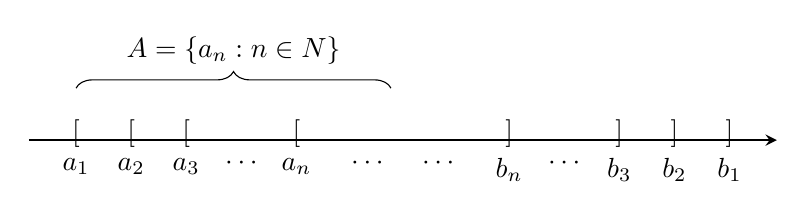
\begin{tikzpicture}[x=1cm, y=1cm]
    \draw[thick, -stealth] (0.25,0) -- (9.75,0);
    \coordinate (aone) at (0.85,0);
    \coordinate (atwo) at (1.55,0);
    \coordinate (athree) at (2.25,0);
    \coordinate (an) at (3.65,0);
    \coordinate (bn) at (6.35,0);
    \coordinate (bthree) at (7.75,0);
    \coordinate (btwo) at (8.45,0);
    \coordinate (bone) at (9.15,0);

    \foreach \p in {aone,atwo,athree,an} {
      \node[anchor=base] at (\p) {$[$};
    }
    \foreach \p in {bn,bthree,btwo,bone} {
      \node[anchor=base] at (\p) {$]$};
    }
    \node at (2.95,-0.3) {$\cdots$};
    \node at (4.55,-0.3) {$\cdots$};
    \node at (5.45,-0.3) {$\cdots$};
    \node at (7.05,-0.3) {$\cdots$};

    \draw[decorate, decoration={brace, amplitude=6pt}]
      (0.85,0.66) -- (4.85,0.66)
      node[midway, above=5pt] {$A=\{a_n:n\in\mathbb{N}\}$};

    \node[below=3pt] at (aone) {$a_1$};
    \node[below=3pt] at (atwo) {$a_2$};
    \node[below=3pt] at (athree) {$a_3$};
    \node[below=3pt] at (an) {$a_n$};
    \node[below=3pt] at (bn) {$b_n$};
    \node[below=3pt] at (bthree) {$b_3$};
    \node[below=3pt] at (btwo) {$b_2$};
    \node[below=3pt] at (bone) {$b_1$};
  \end{tikzpicture}
  \caption{Extremos dos intervalos encaixados e o conjunto
    $A=\{a_n:n\in\mathbb{N}\}$.}
  \label{fig:intervalos-encaixados}
\end{figure}

Considere agora um intervalo particular $I_n=[a_n,b_n]$. Como $x$ é uma cota superior de $A$, temos $a_n\leq x$. O fato de que cada $b_n$ é uma cota superior de $A$ e de que $x$ é a menor cota superior implica $x\leq b_n$.

Assim, $a_n\leq x\leq b_n$, o que significa que $x\in I_n$ para todo $n\in\mathbb{N}$. Consequentemente, $x\in\bigcap_{n=1}^{\infty}I_n$, e a interseção não é vazia.
\end{proof}

\subsection{A Densidade de $\mathbb{Q}$ em $\mathbb{R}$}\label{subsec:densidade-q-r}

O conjunto $\mathbb{Q}$ é uma extensão de $\mathbb{N}$, e $\mathbb{R}$, por sua vez, é uma extensão de $\mathbb{Q}$. Os resultados seguintes indicam como $\mathbb{N}$ e $\mathbb{Q}$ se situam dentro de $\mathbb{R}$.

\index[remissivo]{propriedade!Arquimediana}
\begin{theorem}[Propriedade arquimediana]\label{thm:propriedade-arquimediana}
\begin{enumerate}[label=(\roman*)]
\item Dado qualquer número $x\in\mathbb{R}$, existe $n\in\mathbb{N}$ tal que $n>x$.
\item Dado qualquer número real $y>0$, existe $n\in\mathbb{N}$ tal que $1/n<y$.
\end{enumerate}
\end{theorem}

\begin{proof}
A parte (i) afirma que $\mathbb{N}$ não é limitado superiormente. Pode-se argumentar razoavelmente que não deveríamos ter de provar isso, sobretudo porque decidimos tomar como dadas outras propriedades familiares de $\mathbb{N}$, $\mathbb{Z}$ e $\mathbb{Q}$.

O contra-argumento é que ainda há muito mistério sobre o que são, de fato, os números reais. Até agora, dissemos que $\mathbb{R}$ é uma extensão de $\mathbb{Q}$ que preserva as propriedades algébricas e de ordem dos racionais, mas que também possui a propriedade do supremo formulada no Axioma da Completude. Na ausência de qualquer outra informação sobre $\mathbb{R}$, devemos considerar a possibilidade de que, ao estender $\mathbb{Q}$, tenhamos adquirido inadvertidamente novos números que são cotas superiores de $\mathbb{N}$. Existem, de fato, extensões ordenadas de corpos de $\mathbb{Q}$ que contêm ``números'' maiores que todo número natural. O teorema afirma que os números reais não contêm tais criaturas exóticas. O Axioma da Completude, adotado para preencher as lacunas de $\mathbb{Q}$, implica que $\mathbb{N}$ é um subconjunto ilimitado de $\mathbb{R}$.

Suponha, por contradição, que $\mathbb{N}$ seja limitado superiormente. Pelo Axioma da Completude, $\mathbb{N}$ teria então uma menor cota superior; escreva $\alpha=\sup\mathbb{N}$. O número $\alpha-1$ não é uma cota superior e, portanto, existe $n\in\mathbb{N}$ tal que $\alpha-1<n$. Isso equivale a $\alpha<n+1$. Como $n+1\in\mathbb{N}$, temos uma contradição com o fato de que $\alpha$ deveria ser uma cota superior de $\mathbb{N}$. (Observe que a contradição depende apenas do Axioma da Completude e do fato de $\mathbb{N}$ ser fechado sob a adição.) \index[remissivo]{demonstração!por contradição}

A parte (ii) segue de (i) tomando $x=1/y$.
\end{proof}

Essa propriedade familiar de $\mathbb{N}$ é a chave para um fato extremamente importante sobre a posição de $\mathbb{Q}$ em $\mathbb{R}$.

\index[remissivo]{densidade} \index[remissivo]{densidade!dos racionais}
\begin{theorem}[Densidade de $\mathbb{Q}$ em $\mathbb{R}$]\label{thm:dense-q-r}
Para quaisquer dois números reais $a<b$, existe um número racional $r$ tal que $a<r<b$.
\end{theorem}

\begin{proof}
Um número racional é um quociente de inteiros; portanto, devemos produzir $m\in\mathbb{Z}$ e $n\in\mathbb{N}$ tais que
\[
a<\frac{m}{n}<b.\tag{5}\label{eq:dense-q}
\]
O primeiro passo é escolher o denominador $n$ suficientemente grande para que incrementos consecutivos de tamanho $1/n$ sejam próximos demais para ``pular'' o intervalo $(a,b)$. Usando a propriedade arquimediana, podemos escolher $n\in\mathbb{N}$ tal que
\begin{figure}[htbp]
  \centering
  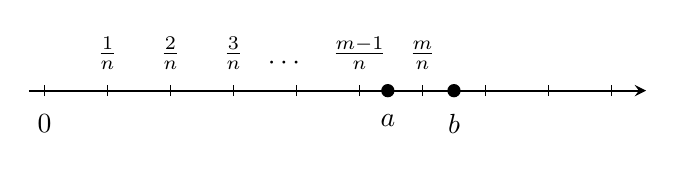
\begin{tikzpicture}[x=0.8cm, y=1cm]
    % Reta graduada em incrementos de tamanho 1/n.
    \draw[thick, -stealth] (-0.25,0) -- (9.55,0);
    \foreach \x in {0,...,9} {
      \draw (\x,-0.07) -- (\x,0.07);
    }

    % Primeiros múltiplos de 1/n.
    \node[above=4pt] at (1,0) {$\frac{1}{n}$};
    \node[above=4pt] at (2,0) {$\frac{2}{n}$};
    \node[above=4pt] at (3,0) {$\frac{3}{n}$};
    \node[above=4pt] at (3.8,0) {$\cdots$};

    % Os dois múltiplos consecutivos que cercam a.
    \node[above=4pt] at (5,0) {$\frac{m-1}{n}$};
    \node[above=4pt] at (6,0) {$\frac{m}{n}$};

    % Pontos a e b na reta.
    \fill (5.45,0) circle (2.4pt);
    \fill (6.50,0) circle (2.4pt);
    \node[below=5pt] at (5.45,0) {$a$};
    \node[below=5pt] at (6.50,0) {$b$};
    \node[below=5pt] at (0,0) {$0$};
  \end{tikzpicture}
  \caption{Múltiplos consecutivos de $1/n$ e existência de um número racional entre $a$ e $b$.}
  \label{fig:densidade-racionais-reta}
\end{figure}

\[
\frac{1}{n}<b-a.\tag{6}\label{eq:one-over-n}
\]

A desigualdade~\eqref{eq:dense-q} equivale a $na<m<nb$. Com $n$ já escolhido, tomamos $m$ como o menor inteiro maior que $na$; isto é, escolhemos $m\in\mathbb{Z}$ de modo que
\[
m-1\leq na<m.\tag{7}\label{eq:m-na}
\]
A desigualdade à direita fornece imediatamente $a<m/n$, que é metade do argumento. Como~\eqref{eq:one-over-n} equivale a $a<b-1/n$, podemos usar a desigualdade à esquerda em~\eqref{eq:m-na} para escrever
\[
\begin{aligned}
m&\leq na+1\\
 &<n\left(b-\frac{1}{n}\right)+1\\
 &=nb.
\end{aligned}
\]
Como $m<nb$ implica $m/n<b$, obtemos $a<m/n<b$, como desejado.
\end{proof}

O \Cref{thm:dense-q-r} é resumido dizendo-se que $\mathbb{Q}$ é \textit{denso} em $\mathbb{R}$. Sem muito esforço, podemos usar esse resultado para mostrar que os números irracionais também são densos em $\mathbb{R}$. \index[remissivo]{números!racionais@\(\mathbb{Q}\)!densidade}

\index[remissivo]{densidade!dos irracionais} \index[remissivo]{números!irracionais!densidade}
\begin{corollary}\label{cor:dense-irracionais}
Dados quaisquer dois números reais $a<b$, existe um número irracional $t$ tal que $a<t<b$.
\end{corollary}

\begin{proof}
Este resultado será demonstrado no Exercício~\Cref{ex:irracionais-densos}.
\end{proof}

\subsection{A Existência de Raízes Quadradas}\label{subsec:raizes-quadradas}

É hora de tratar de uma questão deixada em aberto no \Cref{ex:conjunto-r2-menor-2} e na discussão inicial deste capítulo.

\index[remissivo]{raiz quadrada} \index[remissivo]{raiz quadrada!existência}
\begin{theorem}\label{thm:existencia-sqrt2}
Existe um número real $\alpha\in\mathbb{R}$ tal que $\alpha^2=2$.
\end{theorem}

\begin{proof}
Considere o conjunto
\[
T=\{t\in\mathbb{R}:t^2<2\}
\]
e defina $\alpha=\sup T$. Provaremos que $\alpha^2=2$ excluindo as possibilidades $\alpha^2<2$ e $\alpha^2>2$. Lembre-se de que a definição de $\sup T$ possui duas partes, e ambas serão importantes: mostraremos que $\alpha^2<2$ viola o fato de $\alpha$ ser uma cota superior de $T$, enquanto $\alpha^2>2$ viola o fato de ser a menor cota superior.

Como $1\in T$, temos $\alpha\geq1$; em particular, os denominadores que aparecem abaixo são positivos.

Suponha primeiro que $\alpha^2<2$. Procurando um elemento de $T$ maior que $\alpha$, escrevemos
\[
\begin{aligned}
\left(\alpha+\frac{1}{n}\right)^2
 &=\alpha^2+\frac{2\alpha}{n}+\frac{1}{n^2}\\
 &<\alpha^2+\frac{2\alpha}{n}+\frac{1}{n}\\
 &=\alpha^2+\frac{2\alpha+1}{n}.
\end{aligned}
\]
Como $\alpha^2<2$, há espaço suficiente para acomodar o termo $(2\alpha+1)/n$ e manter o total menor que $2$. Escolha $n_0\in\mathbb{N}$ suficientemente grande para que
\[
\frac{1}{n_0}<\frac{2-\alpha^2}{2\alpha+1}.
\]
Isso implica $(2\alpha+1)/n_0<2-\alpha^2$ e, consequentemente,
\[
\left(\alpha+\frac{1}{n_0}\right)^2<\alpha^2+(2-\alpha^2)=2.
\]
Logo, $\alpha+1/n_0\in T$, contradizendo o fato de que $\alpha$ é uma cota superior de $T$. Concluímos que $\alpha^2<2$ não pode ocorrer.

E quanto ao caso $\alpha^2>2$? Desta vez, escrevemos
\[
\left(\alpha-\frac{1}{n}\right)^2
=\alpha^2-\frac{2\alpha}{n}+\frac{1}{n^2}
>\alpha^2-\frac{2\alpha}{n}.
\]
O restante do argumento é pedido no Exercício~\Cref{ex:finish-sqrt2}.
\end{proof}

Uma pequena modificação dessa demonstração mostra que $\sqrt{x}$ existe para qualquer $x\geq0$. A fórmula binomial, usada para expandir $(\alpha+1/n)^m$, mostra que $\sqrt[m]{x}$ existe para valores arbitrários de $m\in\mathbb{N}$.

\subsection{Lista de Exercícios}\label{subsec:exercicios-consequencias-completude}

\begin{exercise}\label{ex:irracionais-racionais}
Recorde que $\mathbb{I}$ denota o conjunto dos números irracionais. \index[remissivo]{números!irracionais}
\begin{enumerate}[label=\alph*)]
\item Mostre que, se $a,b\in\mathbb{Q}$, então $ab$ e $a+b$ também pertencem a $\mathbb{Q}$.
\item Mostre que, se $a\in\mathbb{Q}$ e $t\in\mathbb{I}$, então $a+t\in\mathbb{I}$ e $at\in\mathbb{I}$, desde que $a\neq0$.
\item A parte (a) pode ser resumida dizendo que $\mathbb{Q}$ é fechado sob a adição e a multiplicação. $\mathbb{I}$ é fechado sob a adição e a multiplicação? Dados dois números irracionais $s$ e $t$, o que podemos dizer sobre $s+t$ e $st$?
\end{enumerate}
\end{exercise}

\begin{exercise}\label{ex:supremo-caracterizacao}
Seja $A\subseteq\mathbb{R}$ não vazio e limitado superiormente, e seja $s\in\mathbb{R}$ tal que, para todo $n\in\mathbb{N}$, $s+1/n$ é uma cota superior de $A$ e $s-1/n$ não é uma cota superior de $A$. Mostre que $s=\sup A$.
\end{exercise}

\begin{exercise}\label{ex:intervalos-abertos-vazios}
Prove que $\bigcap_{n=1}^{\infty}(0,1/n)=\varnothing$. Observe que isso demonstra que os intervalos da propriedade dos intervalos encaixados precisam ser fechados para que a conclusão do teorema seja válida.
\end{exercise}

\begin{exercise}\label{ex:supremo-q-intervalo}
Sejam $a<b$ números reais e considere o conjunto $T=\mathbb{Q}\cap[a,b]$. Mostre que $\sup T=b$.
\end{exercise}

\begin{exercise}\label{ex:irracionais-densos}
Usando o Exercício~\Cref{ex:irracionais-racionais}, prove o Corolário~\Cref{cor:dense-irracionais} considerando os números reais $a-\sqrt{2}$ e $b-\sqrt{2}$.
\end{exercise}

\begin{exercise}\label{ex:conjuntos-densos}
Recorde que um conjunto $B$ é denso em $\mathbb{R}$ se um elemento de $B$ pode ser encontrado entre quaisquer dois números reais $a<b$. Quais dos conjuntos seguintes são densos em $\mathbb{R}$? Em todos os casos, tome $p\in\mathbb{Z}$ e $q\in\mathbb{N}$.
\begin{enumerate}[label=\alph*)]
\item O conjunto de todos os números racionais $p/q$ com $q\leq10$.
\item O conjunto de todos os números racionais $p/q$ com $q$ uma potência de $2$.
\item O conjunto de todos os números racionais $p/q$ com $10|p|\geq q$.
\end{enumerate}
\end{exercise}

\begin{exercise}\label{ex:finish-sqrt2}
Complete a demonstração do \Cref{thm:existencia-sqrt2}, mostrando que a hipótese $\alpha^2>2$ leva a uma contradição com o fato de que $\alpha=\sup T$.
\end{exercise}

\begin{exercise}\label{ex:exemplos-completude}
Dê um exemplo de cada caso ou declare que o pedido é impossível. Quando um pedido for impossível, forneça um argumento convincente para justificar isso.
\begin{enumerate}[label=\alph*)]
\item Dois conjuntos $A$ e $B$ tais que $A\cap B=\varnothing$, $\sup A=\sup B$, $\sup A\notin A$ e $\sup B\notin B$.
\item Uma sequência de intervalos abertos encaixados $J_1\supseteq J_2\supseteq J_3\supseteq\cdots$ cuja interseção seja não vazia, mas contenha apenas um número finito de elementos.
\item Uma sequência de intervalos fechados ilimitados encaixados $L_1\supseteq L_2\supseteq L_3\supseteq\cdots$ tal que $\bigcap_{n=1}^{\infty}L_n=\varnothing$. (Um intervalo fechado ilimitado tem a forma $[a,\infty)=\{x\in\mathbb{R}:x\geq a\}$.)
\end{enumerate}
\end{exercise}


% =====================================================================
% Capítulo 1 — Os Números Reais
% Seção 1.5 Cardinalidade (tradução para PT-BR de Abbott, Understanding
% Analysis, 2ª ed., páginas de índice 37–44 do OCR, incluindo o
% Exercício 1.5.11 no topo da página 44). Este arquivo é incluído via
% \input; não contém preâmbulo nem ambiente document.
% =====================================================================

\index[remissivo]{cardinalidade}
\section{Cardinalidade}\label{sec:cardinalidade}

As aplicações do Axioma da Completude até este ponto serviram, basicamente, para restaurar nossa confiança em propriedades que já acreditávamos conhecer sobre o sistema dos números reais. Uma última consequência da completude, que estamos prestes a explorar, é de natureza muito diferente e, por si só, representa uma descoberta intelectual espantosa. A maneira tradicional como a matemática é feita consiste em um matemático modificando e expandindo o trabalho daqueles que vieram antes. Esse modelo não parece se aplicar a Georg Cantor (1845--1918), ao menos no que diz respeito ao seu trabalho sobre a teoria dos conjuntos infinitos.

No momento, temos uma imagem de $\mathbb{R}$ como consistindo nos números racionais e irracionais, continuamente arrumados ao longo da reta real. Vimos que tanto $\mathbb{Q}$ quanto $\mathbb{I}$ (o conjunto dos irracionais) são densos em $\mathbb{R}$, o que significa que em todo intervalo $(a, b)$ existem tanto números racionais quanto irracionais. Mentalmente, há a tentação de pensar em $\mathbb{Q}$ e $\mathbb{I}$ como estando intrincadamente misturados em proporções iguais, mas esse não é o caso. De uma maneira que Cantor tornou precisa, os números irracionais superam em muito os números racionais na composição da reta real. \index[remissivo]{números!reais@\(\mathbb{R}\)} \index[remissivo]{números!irracionais}

\index[remissivo]{correspondência biunívoca}
\subsection{Correspondência Biunívoca}\label{subsec:correspondencia-biunivoca}

O termo \textit{cardinalidade} é usado em matemática para se referir ao tamanho de um conjunto. As cardinalidades de conjuntos finitos podem ser comparadas simplesmente atribuindo-se um número natural a cada conjunto. O conjunto dos anões da Branca de Neve é menor que o conjunto dos juízes da Suprema Corte dos Estados Unidos porque $7$ é menor que $9$. Mas como poderíamos chegar a essa mesma conclusão sem recorrer a nenhum número? A ideia de Cantor foi tentar colocar os conjuntos em correspondência biunívoca (um-a-um) entre si. Há menos anões que juízes porque, se todos os anões fossem nomeados para a corte simultaneamente, ainda haveria duas cadeiras vazias a preencher. Por outro lado, a cardinalidade da Suprema Corte é a mesma que a cardinalidade do conjunto dos jogadores de um time de beisebol em campo. Isso porque, quando os juízes vão a campo, é possível arranjá-los de modo que haja exatamente um juiz em cada posição. \index[remissivo]{cardinalidade!mesma cardinalidade} \index[remissivo]{correspondência biunívoca}

A vantagem desse método de comparar os tamanhos de conjuntos é que ele funciona igualmente bem para conjuntos infinitos.

\index[remissivo]{função} \index[remissivo]{função!injetora} \index[remissivo]{função!sobrejetora}
\begin{definition}\label{def:injetora-sobrejetora}
Uma função $f \colon A \to B$ é \textit{injetora} (um-a-um) se $a_{1} \neq a_{2}$ em $A$ implica que $f(a_{1}) \neq f(a_{2})$ em $B$. A função $f$ é \textit{sobrejetora} se, dado qualquer $b \in B$, é possível encontrar um elemento $a \in A$ para o qual $f(a) = b$.
\end{definition}

Uma função $f \colon A \to B$ que é simultaneamente injetora e sobrejetora fornece exatamente o que queremos dizer com uma \textit{correspondência biunívoca} entre dois conjuntos. A propriedade de ser injetora significa que dois elementos distintos de $A$ não correspondem ao mesmo elemento de $B$ (não há dois juízes jogando na mesma posição), e a propriedade de ser sobrejetora garante que todo elemento de $B$ corresponde a algum elemento em $A$ (há um juiz em cada posição). \index[remissivo]{correspondência biunívoca}

\index[remissivo]{cardinalidade!mesma cardinalidade}
\begin{definition}\label{def:mesma-cardinalidade}
O conjunto $A$ tem a mesma cardinalidade que $B$ se existe $f \colon A \to B$ que é injetora e sobrejetora. 
Nesse caso, escrevemos $A \sim B$.
\end{definition}

\bigskip 

\begin{example}\label{ex:N-sim-E-Z}
\hfill
\begin{enumerate}[label=\roman*)]
\item Se tomarmos $E = \{2, 4, 6, \dots\}$ como o conjunto dos números naturais pares, então podemos mostrar que $\mathbb{N} \sim E$. Para ver por quê, seja $f \colon \mathbb{N} \to E$ dada por $f(n) = 2n$: \index[remissivo]{números!naturais@\(\mathbb{N}\)}
\[
\begin{array}{lccccc}
\mathbb{N}: & 1 & 2 & 3 & 4 & \cdots \\[0.15cm]
&\updownarrow & \updownarrow & \updownarrow & \updownarrow & \\[0.15cm]
E:&2 & 4 & 6 & 8 & \cdots
\end{array}
\]
É certamente verdade que $E$ é um subconjunto próprio de $\mathbb{N}$ e, por essa razão, pode parecer lógico dizer que $E$ é um conjunto ``menor'' que $\mathbb{N}$. Essa é uma maneira de ver as coisas, mas representa um ponto de vista fortemente enviesado por uma exposição excessiva a conjuntos finitos. A definição de cardinalidade é bastante específica e, desse ponto de vista, $E$ e $\mathbb{N}$ são equivalentes.

\item Para reforçar esse ponto mais uma vez, observe que, embora $\mathbb{N}$ esteja contido em $\mathbb{Z}$ como subconjunto próprio, podemos mostrar que $\mathbb{N} \sim \mathbb{Z}$. Desta vez, seja \index[remissivo]{números!inteiros@\(\mathbb{Z}\)}
\[
f(n) = \begin{cases} (n-1)/2 & \text{se } n \text{ é ímpar}, \\ -n/2 & \text{se } n \text{ é par}, \end{cases}
\]
o que produz a correspondência
\[
\begin{array}{lcccccc}
\mathbb{N}:&1 & 2 & 3 & 4 & 5 & \cdots \\[0.15cm]
&\updownarrow & \updownarrow & \updownarrow & \updownarrow & \updownarrow & \\[0.15cm]
\mathbb{Z}:&0 & -1\ & 1 & -2\ & 2 & \cdots
\end{array}
\]
Os detalhes importantes a verificar são que $f$ não leva dois números naturais distintos ao mesmo elemento de $\mathbb{Z}$ ($f$ é injetora) e que todo elemento de $\mathbb{Z}$ é ``atingido'' por algum número em $\mathbb{N}$ ($f$ é sobrejetora).
\end{enumerate}
\end{example}

\bigskip 

\begin{example}\label{ex:intervalo-sim-R}
Um pouco de cálculo (que não apresentaremos aqui) mostra que a função $f(x) = x/(x^{2} - 1)$ leva o intervalo $(-1, 1)$ sobre $\mathbb{R}$ de maneira injetora e sobrejetora (\Cref{fig:intervalo-sim-R}). Assim, $(-1, 1) \sim \mathbb{R}$. De fato, $(a, b) \sim \mathbb{R}$ para qualquer intervalo $(a, b)$.
\end{example}

\bigskip 

\begin{figure}[htbp]
  \centering
  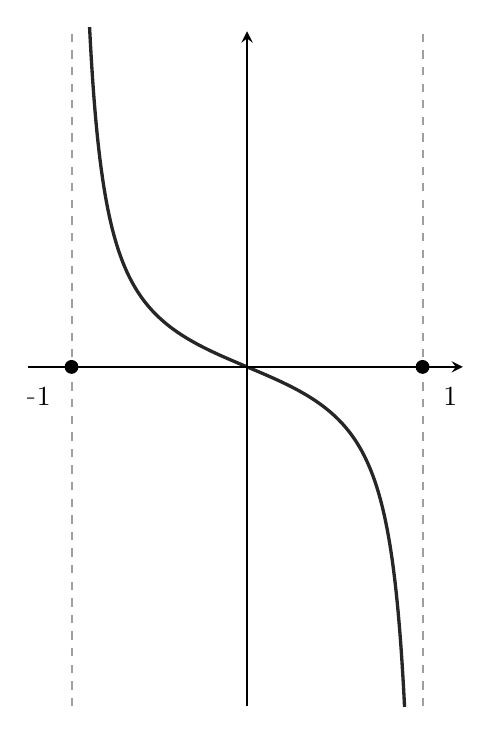
\begin{tikzpicture}
    \begin{axis}[
      width=0.59\textwidth,
      height=10.2cm,
      xmin=-1.25, xmax=1.25,
      ymin=-4.6, ymax=4.6,
      axis lines=none,
      clip=true,
      ticks=none,
      enlargelimits=false,
    ]
      % Gráfico de f(x)=x/(x^2-1), com as duas partes separadas.
      \addplot[
        very thick,
        black!85,
        smooth,
        samples=700,
        domain=-0.995:-0.005,
        unbounded coords=jump,
      ] {x/(x^2-1)};
      \addplot[
        very thick,
        black!85,
        smooth,
        samples=700,
        domain=0.005:0.995,
        unbounded coords=jump,
      ] {x/(x^2-1)};

      % Assíntotas verticais em x=-1 e x=1.
      \draw[dashed, gray!75, line width=0.7pt]
        (axis cs:-1,-4.6) -- (axis cs:-1,4.6);
      \draw[dashed, gray!75, line width=0.7pt]
        (axis cs:1,-4.6) -- (axis cs:1,4.6);

      % Eixos com setas no sentido positivo.
      \draw[thick, ->, >=stealth]
        (axis cs:-1.25,0) -- (axis cs:1.23,0);
      \draw[thick, ->, >=stealth]
        (axis cs:0,-4.6) -- (axis cs:0,4.55);

      % Pontos e rótulos dos extremos do intervalo.
      \fill (axis cs:-1,0) circle (2.5pt);
      \fill (axis cs:1,0) circle (2.5pt);
      \node[below left=4pt] at (axis cs:-1,0) {$-1$};
      \node[below right=4pt] at (axis cs:1,0) {$1$};
    \end{axis}
  \end{tikzpicture}
  \caption{$(-1,1)\sim\mathbb{R}$ usando
    $f(x)=\displaystyle\frac{x}{(x^{2}-1)}$.}
  \label{fig:intervalo-sim-R}
\end{figure}

\index[remissivo]{enumerável} \index[remissivo]{não-enumerável}
\subsection{Conjuntos Enumeráveis}\label{subsec:conjuntos-enumeraveis}

\index[remissivo]{enumerável} \index[remissivo]{não-enumerável}
\begin{definition}\label{def:conjunto-enumeravel}
Um conjunto $A$ é \textit{enumerável} se $\mathbb{N} \sim A$. Um conjunto infinito que não é enumerável é chamado de conjunto \textit{não-enumerável}.
\end{definition}

Do \Cref{ex:N-sim-E-Z}, vemos que tanto $E$ quanto $\mathbb{Z}$ são conjuntos enumeráveis. Colocar um conjunto em correspondência biunívoca com $\mathbb{N}$ significa, na prática, colocar todos os seus elementos em uma lista ou sequência infinitamente longa. Olhando para o \Cref{ex:N-sim-E-Z}, podemos ver que isso foi bastante fácil de fazer para $E$ e exigiu apenas uma modesta reorganização para o conjunto $\mathbb{Z}$. Surge a questão natural de saber se \textit{todos} os conjuntos infinitos são enumeráveis. Dado algum conjunto infinito como $\mathbb{Q}$ ou $\mathbb{R}$, pode parecer que, com engenhosidade suficiente, deveríamos ser capazes de encaixar todos os elementos do nosso conjunto em uma única lista (isto é, em uma correspondência com $\mathbb{N}$). Afinal, essa lista é infinitamente longa, então deveria haver espaço de sobra. Mas, infelizmente, como Hardy observa, ``O assunto [do matemático] é o mais curioso de todos --- não há nenhum outro em que a verdade pregue peças tão estranhas.''

\index[remissivo]{números!racionais@\(\mathbb{Q}\)} \index[remissivo]{números!reais@\(\mathbb{R}\)} \index[remissivo]{enumerável} \index[remissivo]{não-enumerável}
\begin{theorem}\label{thm:Q-enumeravel-R-nao-enumeravel}
\begin{enumerate}[label=(\roman*)]
\item O conjunto $\mathbb{Q}$ é enumerável.
\item O conjunto $\mathbb{R}$ é não-enumerável.
\end{enumerate}
\end{theorem}

\begin{proof}
(i) Defina $A_{1} = \{0\}$ e, para cada $n \geq 2$, seja $A_{n}$ o conjunto dado por
\[
A_{n} = \left\{ \pm \frac{p}{q} : p, q \in \mathbb{N} \text{ com } \frac{p}{q} \text{ na forma irredutível e } p + q = n \right\}.
\]
Os primeiros desses conjuntos são
\[
A_{1} = \{0\}, \quad A_{2} = \left\{ \frac{1}{1}, \frac{-1}{1} \right\}, \quad A_{3} = \left\{ \frac{1}{2}, \frac{-1}{2}, \frac{2}{1}, \frac{-2}{1} \right\},
\]
\[
A_{4} = \left\{ \frac{1}{3}, \frac{-1}{3}, \frac{3}{1}, \frac{-3}{1} \right\}, \quad \text{e} \quad A_{5} = \left\{ \frac{1}{4}, \frac{-1}{4}, \frac{2}{3}, \frac{-2}{3}, \frac{3}{2}, \frac{-3}{2}, \frac{4}{1}, \frac{-4}{1} \right\}.
\]
A observação crucial é que cada $A_{n}$ é \textit{finito} e todo número racional aparece em exatamente um desses conjuntos. Nossa correspondência biunívoca com $\mathbb{N}$ é então obtida listando-se, consecutivamente, os elementos de cada $A_{n}$.
%%Local do conteúdo que falta 
{\setlength{\arraycolsep}{7pt}
\[
\begin{array}{rccccccccccccc}
\mathbb{N}: & 1 & 2 & 3 & 4 & 5 & 6 & 7 & 8 & 9 & 10 & 11 & 12 & \cdots \\[0.15cm]
             & \updownarrow & \updownarrow & \updownarrow & \updownarrow
             & \updownarrow & \updownarrow & \updownarrow & \updownarrow
             & \updownarrow & \updownarrow & \updownarrow & \updownarrow & \\[0.15cm]
\mathbb{Q}: & 0 & \frac{1}{1} & -\frac{1}{1}
             & \frac{1}{2} & -\frac{1}{2}
             & \frac{2}{1} & -\frac{2}{1}
             & \frac{1}{3} & -\frac{1}{3}
             & \frac{3}{1} & -\frac{3}{1}
             & \frac{1}{4} & \cdots \\
             & \multicolumn{1}{c}{\tikz[baseline=-0.5ex]{
                 \draw[decorate, decoration={brace, mirror, amplitude=3pt}]
                   (0,0) -- (0.55,0) node[midway, below=3pt] {$A_{1}$};}}
             & \multicolumn{2}{c}{\tikz[baseline=-0.5ex]{
                 \draw[decorate, decoration={brace, mirror, amplitude=3pt}]
                   (0,0) -- (1.25,0) node[midway, below=3pt] {$A_{2}$};}}
             & \multicolumn{4}{c}{\tikz[baseline=-0.5ex]{
                 \draw[decorate, decoration={brace, mirror, amplitude=3pt}]
                   (0,0) -- (2.9,0) node[midway, below=3pt] {$A_{3}$};}}
             & \multicolumn{4}{c}{\tikz[baseline=-0.5ex]{
                 \draw[decorate, decoration={brace, mirror, amplitude=3pt}]
                   (0,0) -- (2.9,0) node[midway, below=3pt] {$A_{4}$};}}
             & \ldots
\end{array}
\]
}

Como já deve ter sido observado pelo leitor, escrever uma fórmula explícita para essa correspondência 
é uma tarefa bastante árdua, e tentar fazer isto certamente não é um bom uso do nosso tempo. 
O que importa é que fique claro por que todo número racional aparece na 
correspondência exatamente uma vez. 
Dado, digamos, $22/7$, temos que $22/7 \in A_{29}$. Como o conjunto dos 
elementos em $A_{1}, \dots, A_{28}$ é finito, podemos ter certeza de que $22/7$ 
eventualmente é incluído na sequência. O fato de que essa linha de raciocínio 
se aplica a qualquer número racional $p/q$ é a nossa prova de que a correspondência 
é sobrejetora. Para verificar que ela é injetora, observamos que os conjuntos 
$A_{n}$ foram construídos para serem disjuntos, de modo que nenhum número 
racional aparece duas vezes. Isso completa a prova de (i).

\bigskip 

(ii) A segunda afirmação do \Cref{thm:Q-enumeravel-R-nao-enumeravel} é a parte verdadeiramente inesperada, e sua prova é feita por contradição. Suponha que exista, de fato, uma função $f \colon \mathbb{N} \to \mathbb{R}$ que é injetora e sobrejetora. Novamente, o que isso sugere é que é possível enumerar os elementos de $\mathbb{R}$. Se fizermos $x_{1} = f(1)$, $x_{2} = f(2)$, e assim por diante, então nossa suposição de que $f$ é sobrejetora significa que podemos escrever
\[
\mathbb{R} = \{x_{1}, x_{2}, x_{3}, x_{4}, \dots\} \tag{8}\label{eq:enumeracao-R}
\]
e ter a confiança de que todo número real aparece em algum lugar da lista. Usaremos agora a Propriedade dos Intervalos Encaixados (\Cref{thm:intervalos-encaixados}) para produzir um número real que não está lá. \index[remissivo]{propriedade!dos Intervalos Encaixados}

Seja $I_{1}$ um intervalo fechado que não contém $x_{1}$. Em seguida, seja $I_{2}$ um intervalo fechado, contido em $I_{1}$, que não contém $x_{2}$. A existência de tal $I_{2}$ é fácil de verificar. Certamente $I_{1}$ contém dois intervalos fechados menores e disjuntos, e $x_{2}$ só pode estar em um deles. Em geral, dado um intervalo $I_{n}$, construímos $I_{n+1}$ de modo a satisfazer
\begin{enumerate}[label=\roman*)]
\item $I_{n+1} \subseteq I_{n}$ e
\item $x_{n+1} \notin I_{n+1}$.
\end{enumerate}
\vspace*{-1cm}
\begin{figure}[htbp]
  \centering
  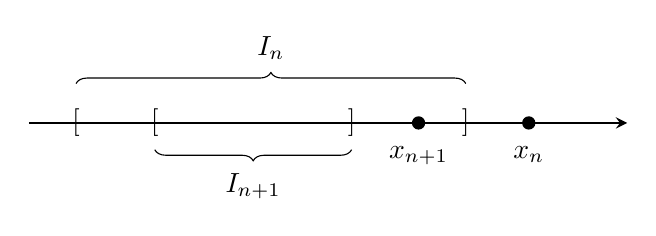
\begin{tikzpicture}[x=1cm, y=1cm]
    % Reta que contém os intervalos e os pontos da lista.
    \draw[thick,-stealth] (-1.35,0) -- (6.25,0);

    % Intervalo maior I_n e intervalo menor I_{n+1}.
    \node[anchor=base] at (-0.75,-0.08) {$[$};
    \node[anchor=base] at (4.20,-0.08) {$]$};
    \node[anchor=base] at (0.25,-0.08) {$[$};
    \node[anchor=base] at (2.75,-0.08) {$]$};

    % Chave superior para I_n.
    \draw[decorate, decoration={brace, amplitude=4pt}]
      (-0.75,0.50) -- (4.20,0.50)
      node[midway, above=5pt] {$I_n$};

    % Chave inferior para I_{n+1}.
    \draw[decorate, decoration={brace, mirror, amplitude=4pt}]
      (0.25,-0.34) -- (2.75,-0.34)
      node[midway, below=5pt] {$I_{n+1}$};

    % Pontos que são excluídos sucessivamente.
    \fill (3.6,0) circle (2.4pt);
    \fill (5.00,0) circle (2.4pt);
    \node[below=5pt] at (3.6,0) {$x_{n+1}$};
    \node[below=5pt] at (5.00,0) {$x_n$};
  \end{tikzpicture}
  \caption{Construção de $I_{n+1}\subseteq I_n$ com
    $x_{n+1}\notin I_{n+1}$.}
  \label{fig:construcao-intervalos-excluindo}
\end{figure}

Consideramos agora a interseção $\bigcap_{n=1}^{\infty} I_{n}$. Se $x_{n_{0}}$ é algum número real da lista em~\eqref{eq:enumeracao-R}, então temos $x_{n_{0}} \notin I_{n_{0}}$, e segue que
\[
x_{n_{0}} \notin \bigcap_{n=1}^{\infty} I_{n}.
\]
Ora, estamos supondo que a lista em~\eqref{eq:enumeracao-R} contém todo número real, e isso leva à conclusão de que
\[
\bigcap_{n=1}^{\infty} I_{n} = \varnothing.
\]
No entanto, a Propriedade dos Intervalos Encaixados afirma que $\bigcap_{n=1}^{\infty} I_{n} \neq \varnothing$. Por essa propriedade, existe ao menos um $x \in \bigcap_{n=1}^{\infty} I_{n}$ que, consequentemente, não pode estar na lista em~\eqref{eq:enumeracao-R}. Essa contradição significa que tal enumeração de $\mathbb{R}$ é impossível, e concluímos que $\mathbb{R}$ é um conjunto \textit{não-enumerável}.
\end{proof}

O que exatamente devemos pensar dessa descoberta? É um exercício importante mostrar que todo subconjunto de um conjunto enumerável deve ser enumerável ou finito. Isso não deve ser muito surpreendente. Se um conjunto pode ser arranjado em uma única lista, então remover alguns elementos dessa lista resulta em outra lista (mais curta, e possivelmente com fim). Isso significa que os conjuntos enumeráveis são o menor tipo de conjunto infinito. Qualquer coisa menor é ainda enumerável ou finita. \index[remissivo]{conjunto!subconjunto} \index[remissivo]{enumerável!subconjunto}

A força do \Cref{thm:Q-enumeravel-R-nao-enumeravel} é que a cardinalidade de $\mathbb{R}$ é, falando informalmente, um tipo maior de infinito. Os números reais superam tanto os números naturais em quantidade que não há como mapear $\mathbb{N}$ sobre $\mathbb{R}$. Não importa como tentemos, há sempre números reais que irão ficar de fora
de qualquer emparelhamento. O conjunto $\mathbb{Q}$, por outro lado, é enumerável. No que diz respeito a conjuntos infinitos, é tão pequeno quanto possível. O que isso implica sobre o conjunto $\mathbb{I}$ dos números irracionais? Imitando a demonstração de que $\mathbb{N} \sim \mathbb{Z}$, podemos provar que a união de dois conjuntos enumeráveis deve ser enumerável. Como $\mathbb{R} = \mathbb{Q} \cup \mathbb{I}$, segue que $\mathbb{I}$ não pode ser enumerável, pois caso contrário $\mathbb{R}$ o seria. A conclusão inescapável é que, apesar do fato de termos encontrado tão poucos deles, os números irracionais formam um subconjunto muito maior de $\mathbb{R}$ do que $\mathbb{Q}$. \index[remissivo]{números!irracionais} \index[remissivo]{não-enumerável}

As propriedades dos conjuntos enumeráveis descritas nestas notas 
serão úteis para vários exercícios ao longo do curso. 
Para referências futuras, vamos enunciar algumas proposições 
e esboçar suas provas nos exercícios que se seguem.

\index[remissivo]{enumerável!subconjunto} \index[remissivo]{conjunto!subconjunto}
\begin{theorem}\label{thm:subconjunto-enumeravel}
Se $A \subseteq B$ e $B$ é enumerável, então $A$ é enumerável ou finito.
\end{theorem}

\index[remissivo]{enumerável!união} \index[remissivo]{conjunto!união}
\begin{theorem}\label{thm:uniao-enumeravel}
\begin{enumerate}[label=\roman*)]
\item Se $A_{1}, A_{2}, \ldots, A_{m}$ são conjuntos enumeráveis, então a união $A_{1} \cup A_{2} \cup \cdots \cup A_{m}$ é enumerável.
\item Se $A_{n}$ é um conjunto enumerável para cada $n \in \mathbb{N}$, então $\bigcup_{n=1}^{\infty} A_{n}$ é enumerável.
\end{enumerate}
\end{theorem}

\subsection{Lista de Exercícios}\label{subsec:exercicios-cardinalidade}

\begin{exercise}\label{ex:completar-prova-subconjunto}
Complete a seguinte prova do \Cref{thm:subconjunto-enumeravel}.

Suponha que $B$ é um conjunto enumerável. Assim, existe $f \colon \mathbb{N} \to B$, que é injetora e sobrejetora. Seja $A \subseteq B$ um subconjunto infinito de $B$. Devemos mostrar que $A$ é enumerável.

Seja $n_{1} = \min\{n \in \mathbb{N} : f(n) \in A\}$. Como início de uma definição de $g \colon \mathbb{N} \to A$, faça $g(1) = f(n_{1})$. Mostre como continuar esse processo indutivamente para produzir uma função $g$ injetora de $\mathbb{N}$ sobre $A$. \index[remissivo]{indução matemática}
\end{exercise}

\begin{exercise}\label{ex:falha-prova-Q-nao-enumeravel}
Revise a prova do \Cref{thm:Q-enumeravel-R-nao-enumeravel}, parte (ii), mostrando que $\mathbb{R}$ é não-enumerável, e então encontre a falha na seguinte prova errônea de que $\mathbb{Q}$ é não-enumerável:

Suponha, por contradição, que $\mathbb{Q}$ é enumerável. Assim, podemos escrever $\mathbb{Q} = \{r_{1}, r_{2}, r_{3}, \dots\}$ e, como antes, construir uma sequência encaixada de intervalos fechados com $r_{n} \notin I_{n}$. Nossa construção implica $\bigcap_{n=1}^{\infty} I_{n} = \varnothing$, enquanto a Propriedade dos Intervalos Encaixados implica $\bigcap_{n=1}^{\infty} I_{n} \neq \varnothing$. Essa contradição implica que $\mathbb{Q}$ deve, portanto, ser não-enumerável.
\end{exercise}


\break 

\begin{exercise}\label{ex:prova-uniao-enumeravel}
Use o roteiro a seguir para fornecer provas das afirmações do \Cref{thm:uniao-enumeravel}.
\begin{enumerate}[label=\alph*)]
\item Primeiro, prove a afirmação (i) para dois conjuntos enumeráveis, $A_{1}$ e $A_{2}$. O \Cref{ex:N-sim-E-Z} (ii) pode ser uma referência útil. Algumas tecnicidades podem ser evitadas substituindo primeiro $A_{2}$ pelo conjunto $B_{2} = A_{2} \setminus A_{1} = \{x \in A_{2} : x \notin A_{1}\}$. O propósito disso é que a união $A_{1} \cup B_{2}$ é igual a $A_{1} \cup A_{2}$ e os conjuntos $A_{1}$ e $B_{2}$ são disjuntos. (O que acontece se $B_{2}$ é finito?)

Agora, explique como a afirmação mais geral em (i) segue.
\item Explique por que a indução \textit{não pode} ser usada para provar a parte (ii) do \Cref{thm:uniao-enumeravel} a partir da parte (i).
\item Mostre como arranjar $\mathbb{N}$ na matriz bidimensional
\[
\begin{array}{ccccc}
1 & 2 & 4 & 7 & \cdots \\
3 & 5 & 8 & \vdots & \\
6 & 9 & \vdots & & \\
10 & \vdots & & &
\end{array}
\]
e percorrer suas diagonais leva a uma prova do \Cref{thm:uniao-enumeravel} (ii).
\end{enumerate}
\end{exercise}

\begin{exercise}\label{ex:intervalos-cardinalidade-R}
\begin{enumerate}[label=\alph*)]
\item Mostre que $(a, b) \sim \mathbb{R}$ para qualquer intervalo $(a, b)$.
\item Mostre que um intervalo ilimitado como $(a, \infty) = \{x : x > a\}$ também tem a mesma cardinalidade que $\mathbb{R}$.
\item Usar intervalos abertos torna mais conveniente produzir as funções injetoras e sobrejetoras necessárias, mas isso não é realmente necessário. Mostre que $[0, 1) \sim (0, 1)$ exibindo uma função injetora e sobrejetora entre os dois conjuntos.
\end{enumerate}
\end{exercise}

\begin{exercise}\label{ex:equivalencia-cardinalidade}
\begin{enumerate}[label=\alph*)]
\item Por que $A \sim A$ para todo conjunto $A$?
\item Dados conjuntos $A$ e $B$, explique por que $A \sim B$ é equivalente a afirmar $B \sim A$.
\item Para três conjuntos $A$, $B$ e $C$, mostre que $A \sim B$ e $B \sim C$ implicam $A \sim C$. Essas três propriedades são o que se quer dizer ao afirmar que $\sim$ é uma \textit{relação de equivalência}.
\end{enumerate}
\end{exercise}

\begin{exercise}\label{ex:intervalos-abertos-disjuntos}
\begin{enumerate}[label=\alph*)]
\item Dê um exemplo de uma coleção enumerável de intervalos abertos disjuntos.
\item Dê um exemplo de uma coleção não-enumerável de intervalos abertos disjuntos, ou argumente que tal coleção não existe.
\end{enumerate}
\end{exercise}

\begin{exercise}\label{ex:quadrado-unitario}
Considere o intervalo aberto $(0, 1)$ e seja $S$ o conjunto de pontos do quadrado unitário aberto; isto é, $S = \{(x, y) : 0 < x, y < 1\}$.
\begin{enumerate}[label=\alph*)]
\item Encontre uma função injetora que mapeia $(0, 1)$ em $S$, mas não necessariamente sobre $S$. (Isso é fácil.)
\item Use o fato de que todo número real tem uma expansão decimal para produzir uma função injetora que mapeia $S$ em $(0, 1)$. Discuta se a função formulada é sobrejetora. (Tenha em mente que qualquer expansão decimal finita, como $0{,}235$, representa o mesmo número real que $0{,}234999\ldots$)
\end{enumerate}
O Teorema de Schröder--Bernstein, discutido no \Cref{ex:schroder-bernstein}, pode agora ser aplicado para concluir que $(0, 1) \sim S$. \index[remissivo]{teorema!de Schröder--Bernstein}
\end{exercise}

\begin{exercise}\label{ex:conjunto-somas-limitadas}
Seja $B$ um conjunto de números reais positivos com a propriedade de que somar qualquer subconjunto finito de elementos de $B$ resulta sempre em uma soma menor ou igual a $2$. Mostre que $B$ deve ser finito ou enumerável.
\end{exercise}

\begin{exercise}\label{ex:numeros-algebricos}
Um número real $x \in \mathbb{R}$ é chamado \textit{algébrico} se existem inteiros $a_{0}, a_{1}, a_{2}, \ldots, a_{n} \in \mathbb{Z}$, nem todos nulos, tais que \index[remissivo]{números!algébrico} \index[remissivo]{números!reais@\(\mathbb{R}\)}
\[
a_{n} x^{n} + a_{n-1} x^{n-1} + \cdots + a_{1} x + a_{0} = 0.
\]
Dito de outra forma, um número real é algébrico se é raiz de um polinômio com coeficientes inteiros. Números reais que não são algébricos são chamados de números \textit{transcendentes}. Releia o último parágrafo da \Cref{sec:irracionalidade-sqrt2}. A questão final colocada ali está intimamente relacionada à questão de saber se números transcendentes existem. \index[remissivo]{números!transcendente}
\begin{enumerate}[label=\alph*)]
\item Mostre que $\sqrt{2}$, $\sqrt[3]{2}$ e $\sqrt{3} + \sqrt{2}$ são algébricos.
\item Fixe $n \in \mathbb{N}$ e seja $A_{n}$ o conjunto dos números algébricos obtidos como raízes de polinômios com coeficientes inteiros que têm grau $n$. Usando o fato de que todo polinômio tem um número finito de raízes, mostre que $A_{n}$ é enumerável. \index[remissivo]{números!algébrico!enumerabilidade} \index[remissivo]{enumerável}
\item Agora, argumente que o conjunto de todos os números algébricos é enumerável. O que podemos concluir sobre o conjunto dos números transcendentes?
\end{enumerate}
\end{exercise}

\begin{exercise}\label{ex:corte-nao-enumeravel}
\begin{enumerate}[label=\alph*)]
\item Seja $C \subseteq [0, 1]$ não-enumerável. Mostre que existe $a \in (0, 1)$ tal que $C \cap [a, 1]$ é não-enumerável.
\item Agora seja $A$ o conjunto de todos os $a \in (0, 1)$ tais que $C \cap [a, 1]$ é não-enumerável, e faça $\alpha = \sup A$. O conjunto $C \cap [\alpha, 1]$ é não-enumerável?
\item A afirmação em (a) permanece verdadeira se ``não-enumerável'' for substituído por ``infinito''?
\end{enumerate}
\end{exercise}

\index[remissivo]{teorema!de Schröder--Bernstein}
\begin{exercise}[Teorema de Schröder--Bernstein]\label{ex:schroder-bernstein}
Suponha que existe uma função injetora $f \colon X \to Y$ e outra função injetora $g \colon Y \to X$. Siga os passos para mostrar que existe uma função $h \colon X \to Y$ injetora e sobrejetora e, portanto, $X \sim Y$.

A estratégia é particionar $X$ e $Y$ em componentes
\[
X = A \cup A' \quad \text{e} \quad Y = B \cup B'
\]
com $A \cap A' = \varnothing$ e $B \cap B' = \varnothing$, de tal modo que $f$ mapeia $A$ sobre $B$, e $g$ mapeia $B'$ sobre $A'$.
\begin{enumerate}[label=\alph*)]
\item Explique como alcançar isso levaria a uma prova de que $X \sim Y$.
\item Faça $A_{1} = X \setminus g(Y) = \{x \in X : x \notin g(Y)\}$ (o que acontece se $A_{1} = \varnothing$?) e defina indutivamente uma sequência de conjuntos fazendo $A_{n+1} = g(f(A_{n}))$. Mostre que $\{A_{n} : n \in \mathbb{N}\}$ é uma coleção disjunta dois a dois de subconjuntos de $X$, enquanto $\{f(A_{n}) : n \in \mathbb{N}\}$ é uma coleção semelhante em $Y$.
\item Seja $A = \bigcup_{n=1}^{\infty} A_{n}$ e $B = \bigcup_{n=1}^{\infty} f(A_{n})$. Mostre que $f$ mapeia $A$ sobre $B$.
\item Seja $A' = X \setminus A$ e $B' = Y \setminus B$. Mostre que $g$ mapeia $B'$ sobre $A'$.
\end{enumerate}
\end{exercise}


% =====================================================================
% Capítulo 1 — Os Números Reais
% Seção 1.6 (tradução para PT-BR de Abbott, Understanding Analysis,
% 2ª ed., páginas 44–47 do OCR). Este arquivo deve ser incluído via
% \input; o título do capítulo é declarado no arquivo principal.
% =====================================================================

\index[remissivo]{teorema!de Cantor}
\section{O Teorema de Cantor}\label{sec:teorema-cantor}

O trabalho de Cantor sobre a teoria dos conjuntos infinitos estende-se muito além das conclusões do \Cref{thm:Q-enumeravel-R-nao-enumeravel}. Embora tenha sido inicialmente recebido com resistência, seu ataque criativo e persistente nessa área acabou por produzir uma revolução na teoria dos conjuntos e uma mudança de paradigma na maneira como os matemáticos passaram a entender o infinito.

\index[remissivo]{método de diagonalização}
\subsection{O Método de Diagonalização de Cantor}\label{subsec:metodo-diagonalizacao}

Cantor publicou, em 1874, sua descoberta de que $\mathbb{R}$ é não-enumerável. Embora tenha recebido certo polimento moderno, o argumento apresentado no \Cref{thm:Q-enumeravel-R-nao-enumeravel} (ii) é, na verdade, bastante semelhante àquele encontrado originalmente por Cantor. Em 1891, Cantor ofereceu outra demonstração desse mesmo fato, surpreendente em sua simplicidade. Ela se apoia nas representações decimais dos números reais, que aceitaremos e usaremos sem quaisquer definições formais.

\index[remissivo]{não-enumerável} \index[remissivo]{números!reais@\(\mathbb{R}\)}
\begin{theorem}\label{thm:01-nao-enumeravel}
O intervalo aberto $(0, 1) = \{ x \in \mathbb{R} : 0 < x < 1 \}$ é não-enumerável.
\end{theorem}

\begin{exercise}\label{ex:01-iff-R-nao-enumeravel}
Mostre que $(0, 1)$ é não-enumerável se, e somente se, $\mathbb{R}$ é não-enumerável. Isso mostra que o \Cref{thm:01-nao-enumeravel} é equivalente ao \Cref{thm:Q-enumeravel-R-nao-enumeravel}.
\end{exercise}

\begin{proof}
Como no \Cref{thm:Q-enumeravel-R-nao-enumeravel}, procedemos por contradição e supomos que exista, de fato, uma função $f \colon \mathbb{N} \to (0, 1)$ que seja injetora e sobrejetora. Para cada $m \in \mathbb{N}$, $f(m)$ é um número real entre $0$ e $1$, e o representamos usando a notação decimal
\[
f(m) = 0{,}a_{m1} a_{m2} a_{m3} a_{m4} a_{m5} \dots
\]
O que se quer dizer aqui é que, para cada $m, n \in \mathbb{N}$, $a_{mn}$ é um 
dígito do conjunto $\{0, 1, 2, \dots, 9\}$ que 
representa o $n$-ésimo dígito da expansão decimal de $f(m)$. 
A correspondência biunívoca entre $\mathbb{N}$ e $(0, 1)$ pode ser 
resumida na seguinte matriz 

\[
\renewcommand{\arraystretch}{1.5}%
\setlength{\arraycolsep}{0.3em}%
\begin{array}{c@{\qquad}c@{\qquad}r@{\;\;}c@{\;\;}*{6}{c@{\qquad}}c}
\mathbb{N} & & (0,1) \\
\cline{1-10}
1 & \longleftrightarrow & f(1) & = & .\,\boldsymbol{a_{11}} & a_{12} & a_{13} & a_{14} & a_{15} & a_{16} & \dots \\
2 & \longleftrightarrow & f(2) & = & .\,a_{21} & \boldsymbol{a_{22}} & a_{23} & a_{24} & a_{25} & a_{26} & \dots \\
3 & \longleftrightarrow & f(3) & = & .\,a_{31} & a_{32} & \boldsymbol{a_{33}} & a_{34} & a_{35} & a_{36} & \dots \\
4 & \longleftrightarrow & f(4) & = & .\,a_{41} & a_{42} & a_{43} & \boldsymbol{a_{44}} & a_{45} & a_{46} & \dots \\
5 & \longleftrightarrow & f(5) & = & .\,a_{51} & a_{52} & a_{53} & a_{54} & \boldsymbol{a_{55}} & a_{56} & \dots \\
6 & \longleftrightarrow & f(6) & = & .\,a_{61} & a_{62} & a_{63} & a_{64} & a_{65} & \boldsymbol{a_{66}} & \dots \\
\vdots & \vdots & \vdots & & \vdots & \vdots & \vdots & \vdots & \vdots & \vdots & \ddots
\end{array}
\]
A hipótese fundamental acerca dessa correspondência é que \textit{todo} número real em $(0, 1)$ aparece 
em alguma posição desta lista.

Chegamos agora à pérola do argumento. Defina um número real $x \in (0, 1)$ com expansão decimal $x = 0{,}b_{1} b_{2} b_{3} b_{4} \dots$ usando a regra \index[remissivo]{método de diagonalização}
\[
b_{n} = \begin{cases} 2 & \text{se } a_{nn} \neq 2, \\ 3 & \text{se } a_{nn} = 2. \end{cases}
\]
Sejamos claros a esse respeito. Para calcular o dígito $b_{1}$, olhamos para o dígito $a_{11}$ no canto superior esquerdo da matriz. Se $a_{11} = 2$, então escolhemos $b_{1} = 3$; caso contrário, tomamos $b_{1} = 2$.

\begin{exercise}\label{ex:passos-diagonalizacao}
\begin{enumerate}[label=\alph*)]
\item Explique por que o número real $x = 0{,}b_{1} b_{2} b_{3} b_{4} \dots$ não pode ser $f(1)$.
\item Agora, explique por que $x \neq f(2)$ e, em geral, por que $x \neq f(n)$ para qualquer $n \in \mathbb{N}$.
\item Aponte a contradição que surge dessas observações e conclua que $(0, 1)$ é não-enumerável.
\end{enumerate}
\end{exercise}
\end{proof}

\begin{exercise}\label{ex:objecoes-diagonalizacao}
Forneça refutações às seguintes objeções à demonstração do \Cref{thm:01-nao-enumeravel}.
\begin{enumerate}[label=\alph*)]
\item Todo número racional possui uma expansão decimal, de modo que poderíamos aplicar esse mesmo argumento para mostrar que o conjunto dos números racionais entre $0$ e $1$ é não-enumerável. No entanto, como sabemos que qualquer subconjunto de $\mathbb{Q}$ deve ser contável, a demonstração do \Cref{thm:01-nao-enumeravel} deve ter alguma falha.
\item Alguns números possuem \textit{duas} representações decimais diferentes. Especificamente, qualquer expansão decimal finita pode também ser escrita com $9$s periódicos. Por exemplo, $1/2$ pode ser escrito como $0{,}5$ ou como $0{,}4999\dots$. Isso não causa problemas?
\end{enumerate}
\end{exercise}

\begin{exercise}\label{ex:sequencias-01-nao-enumeravel}
Seja $S$ o conjunto constituído por todas as sequências de $0$s e $1$s. Observe que $S$ não é uma sequência particular, mas sim um conjunto grande, cujos elementos são sequências; a saber,
\[
S = \{ (a_{1}, a_{2}, a_{3}, \ldots) : a_{n} = 0 \text{ ou } 1 \}.
\]
Como exemplo, a sequência $(1, 0, 1, 0, 1, 0, 1, 0, \ldots)$ é um elemento de $S$, assim como a sequência $(1, 1, 1, 1, 1, 1, \ldots)$.

Apresente um argumento rigoroso mostrando que $S$ é não-enumerável.
\end{exercise}

Depois de distinguir entre a infinidade contável de $\mathbb{N}$ e a infinidade não-enumerável de $\mathbb{R}$, uma nova questão que ocupou Cantor foi a de saber se existiria uma infinidade ``acima'' da de $\mathbb{R}$. Este é um território logicamente traiçoeiro. O mesmo cuidado que tivemos ao definir a relação ``ter a mesma cardinalidade que'' precisa ser dedicado à definição de relações como ``ter cardinalidade maior que'' ou ``ter cardinalidade menor ou igual a''. Não obstante, sem nos sobrecarregarmos demais com definições formais, o próximo resultado nos dá uma noção bastante clara de que existe uma hierarquia de conjuntos infinitos que se estende muito além do contínuo de $\mathbb{R}$.

\index[remissivo]{conjunto!das partes}
\subsection{Conjunto das Partes e o Teorema de Cantor}\label{subsec:conjunto-partes}

\index[remissivo]{conjunto!das partes} \index[remissivo]{conjunto!subconjunto}
\begin{definition}[Conjunto das partes]\label{def:conjunto-partes}
Dado um conjunto $A$, o \textit{conjunto das partes} $\mathcal{P}(A)$ (em inglês, \textit{power set}) refere-se à coleção de todos os subconjuntos de $A$. É importante entender que $\mathcal{P}(A)$ é, ele próprio, considerado um conjunto, cujos elementos são os diferentes subconjuntos possíveis de $A$.
\end{definition}

\begin{exercise}\label{ex:partes-abc}
\begin{enumerate}[label=\alph*)]
\item Seja $A = \{a, b, c\}$. Liste os oito elementos de $\mathcal{P}(A)$. (Não se esqueça de que $\varnothing$ é considerado subconjunto de todo conjunto.)
\item Se $A$ é finito com $n$ elementos, mostre que $\mathcal{P}(A)$ tem $2^{n}$ elementos.
\end{enumerate}
\end{exercise}

\begin{exercise}\label{ex:aplicacoes-injetoras-PA}
\begin{enumerate}[label=\alph*)]
\item Usando o conjunto particular $A = \{a, b, c\}$, exiba duas aplicações injetoras diferentes de $A$ em $\mathcal{P}(A)$.
\item Tomando $C = \{1, 2, 3, 4\}$, produza um exemplo de aplicação injetora $g \colon C \to \mathcal{P}(C)$.
\item Explique por que, nos itens (a) e (b), é impossível construir aplicações que sejam sobrejetoras.
\end{enumerate}
\end{exercise}

O Teorema de Cantor afirma que o fenômeno do \Cref{ex:aplicacoes-injetoras-PA} vale tanto para conjuntos infinitos quanto para conjuntos finitos. Enquanto mapear $A$ em $\mathcal{P}(A)$ é algo bastante simples, encontrar uma aplicação sobrejetora é impossível.

\index[remissivo]{teorema!de Cantor} \index[remissivo]{conjunto!das partes}
\begin{theorem}[Teorema de Cantor]\label{thm:cantor}
Dado um conjunto $A$ qualquer, não existe função $f \colon A \to \mathcal{P}(A)$ que seja sobrejetora. \index[remissivo]{função!sobrejetora} \index[remissivo]{conjunto!das partes}
\end{theorem}

\begin{proof}
Esta demonstração, como outras do mesmo tipo, é indireta. Assim, suponha, por contradição, que $f \colon A \to \mathcal{P}(A)$ é sobrejetora. Ao contrário da situação usual, em que temos conjuntos de números como domínio e contradomínio, $f$ é uma correspondência entre um conjunto e seu conjunto das partes. Para cada elemento $a \in A$, $f(a)$ é um subconjunto particular de $A$.

A suposição de que $f$ é sobrejetora significa que todo subconjunto de $A$ aparece como $f(a)$ para algum $a \in A$. Para chegar a uma contradição, produziremos um subconjunto $B \subseteq A$ que não é igual a $f(a)$ para nenhum $a \in A$.

Construímos $B$ usando a regra a seguir. Para cada elemento $a \in A$, considere o subconjunto $f(a)$. Esse subconjunto de $A$ pode conter o elemento $a$ ou não; isso depende da função $f$. Se $f(a)$ não contém $a$, então incluímos $a$ em nosso conjunto $B$. Mais precisamente, seja
\[
B = \{ a \in A : a \notin f(a) \}.
\]

\begin{exercise}\label{ex:conjunto-B-exemplo}
Retorne às funções particulares construídas no \Cref{ex:aplicacoes-injetoras-PA} e construa o subconjunto $B$ resultante do uso da regra anterior. Em cada caso, observe que $B$ não está na imagem da função usada.
\end{exercise}

Concentremo-nos agora no argumento geral. Como supusemos que nossa função $f \colon A \to \mathcal{P}(A)$ é sobrejetora, deve-se ter $B = f(a')$ para algum $a' \in A$. A contradição surge quando consideramos se $a'$ é ou não um elemento de $B$.

\begin{exercise}\label{ex:contradicao-B}
\begin{enumerate}[label=\alph*)]
\item Primeiro, mostre que o caso $a' \in B$ leva a uma contradição.
\item Agora, termine o argumento mostrando que o caso $a' \notin B$ é igualmente inaceitável.
\end{enumerate}
\end{exercise}
\end{proof}

Para ter uma noção inicial de sua ampla significância, apliquemos esse resultado ao conjunto dos números naturais. O \Cref{thm:cantor} afirma que não existe função sobrejetora de $\mathbb{N}$ em $\mathcal{P}(\mathbb{N})$; em outras palavras, o conjunto das partes dos números naturais é não-enumerável. Como a cardinalidade desse conjunto não-enumerável recém-descoberto se compara à do conjunto não-enumerável dos números reais? \index[remissivo]{conjunto!das partes} \index[remissivo]{não-enumerável}

\begin{exercise}\label{ex:PN-sim-R}
Usando as diversas ferramentas e técnicas desenvolvidas nas duas últimas seções (incluindo os exercícios da \Cref{sec:cardinalidade}), apresente um argumento convincente mostrando que $\mathcal{P}(\mathbb{N}) \sim \mathbb{R}$.
\end{exercise}

\begin{exercise}\label{ex:cardinalidades-conjuntos-funcoes}
Como exercício final, responda a cada uma das questões a seguir estabelecendo uma correspondência biunívoca com um conjunto de cardinalidade conhecida.
\begin{enumerate}[label=\alph*)]
\item O conjunto de todas as funções de $\{0, 1\}$ em $\mathbb{N}$ é contável ou não-enumerável?
\item O conjunto de todas as funções de $\mathbb{N}$ em $\{0, 1\}$ é contável ou não-enumerável?
\item Dado um conjunto $B$, um subconjunto $\mathcal{A}$ de $\mathcal{P}(B)$ é chamado de \textit{anticadeia} se nenhum elemento de $\mathcal{A}$ é subconjunto de qualquer outro elemento de $\mathcal{A}$. O conjunto $\mathcal{P}(\mathbb{N})$ contém uma anticadeia não-enumerável?
\end{enumerate}
\end{exercise}

\section{A Escala dos Infinitos}\label{sec:epilogo}

A relação ``ter a mesma cardinalidade'' é uma \textit{relação de equivalência} (veja o \Cref{ex:equivalencia-cardinalidade}); isso significa, grosso modo, que todos os conjuntos do universo matemático podem ser organizados em grupos disjuntos de acordo com seu tamanho. Dois conjuntos pertencem ao mesmo grupo, ou \textit{classe de equivalência}, se, e somente se, têm a mesma cardinalidade. Assim, $\mathbb{N}$, $\mathbb{Z}$ e $\mathbb{Q}$ ficam reunidos em uma classe com todos os outros conjuntos enumeráveis, enquanto $\mathbb{R}$ pertence a outra classe, que inclui os intervalos $(a, b)$ e também $\mathcal{P}(\mathbb{N})$. Uma consequência do Teorema de Cantor é que $\mathcal{P}(\mathbb{R})$ --- o conjunto de todos os subconjuntos de $\mathbb{R}$ --- pertence a uma classe diferente daquela de $\mathbb{R}$, e não há motivo para parar por aí. O conjunto dos subconjuntos de $\mathcal{P}(\mathbb{R})$, isto é, $\mathcal{P}(\mathcal{P}(\mathbb{R}))$, pertence a uma classe ainda distinta, e esse processo prossegue indefinidamente. \index[remissivo]{teorema!de Cantor} \index[remissivo]{conjunto!das partes}

Depois de dividir o universo dos conjuntos em grupos disjuntos, seria conveniente associar um ``número'' a cada coleção, que pudesse ser usado da mesma maneira que os números naturais são usados para indicar os tamanhos de conjuntos finitos. Dado um conjunto $X$, existe algo chamado \textit{número cardinal} de $X$, denotado por $\operatorname{card} X$, que se comporta de maneira muito semelhante. Por exemplo, dois conjuntos $X$ e $Y$ satisfazem $\operatorname{card} X = \operatorname{card} Y$ se, e somente se, $X \sim Y$. (Definir rigorosamente $\operatorname{card} X$ requer uma teoria dos conjuntos considerável. Uma maneira de fazer isso é definir $\operatorname{card} X$ como um conjunto muito particular que pode ser encontrado de maneira única na mesma classe de equivalência que $X$.) \index[remissivo]{números!cardinal} \index[remissivo]{cardinalidade!número cardinal}

Ao retomarmos o Teorema de Cantor, temos a forte impressão de que existe uma \textit{ordem} entre os tamanhos dos conjuntos infinitos, a qual deveria se refletir em nosso novo sistema de números cardinais. Mais precisamente, se for possível mapear um conjunto $X$ em $Y$ de maneira injetora, queremos que $\operatorname{card} X \leq \operatorname{card} Y$. Escrever a desigualdade estrita $\operatorname{card} X < \operatorname{card} Y$ deve indicar que é possível mapear $X$ em $Y$, mas que não ocorre $X \sim Y$. Reescrito nessa notação, o Teorema de Cantor afirma que, para todo conjunto $A$, \index[remissivo]{números!cardinal} \index[remissivo]{função!injetora}
\[
\operatorname{card} A < \operatorname{card} \mathcal{P}(A).
\]

Há detalhes importantes a resolver. Surge uma espécie de problema metafísico quando percebemos que uma consequência do Teorema de Cantor é a inexistência de um conjunto ``maior de todos''. Uma afirmação como ``Seja $U$ o conjunto de todas as coisas possíveis'' é paradoxal, pois imediatamente obtemos $\operatorname{card} U < \operatorname{card} \mathcal{P}(U)$ e, portanto, o conjunto $U$ não contém tudo aquilo que se anunciava que ele conteria. Questões como essa são resolvidas, em última análise, impondo algumas restrições ao que pode ser considerado um conjunto. À medida que a teoria dos conjuntos foi formalizada, os axiomas tiveram de ser elaborados de modo que objetos como $U$ simplesmente não fossem permitidos. Um problema mais concreto que exige atenção é demonstrar que nossa definição de ``$\leq$'' entre números cardinais realmente define uma ordem. Isso envolve mostrar que os números cardinais possuem uma propriedade análoga à dos números reais: se $\operatorname{card} X \leq \operatorname{card} Y$ e $\operatorname{card} Y \leq \operatorname{card} X$, então $\operatorname{card} X = \operatorname{card} Y$. No fim, isso se reduz a provar que, se existe uma função injetora $f \colon X \to Y$ e existe uma função injetora $g \colon Y \to X$, então é possível encontrar uma função $h \colon X \to Y$ que seja simultaneamente injetora e sobrejetora. Uma demonstração desse fato escapou a Cantor, mas foi fornecida independentemente por Ernst Schröder (em 1896) e Felix Bernstein (em 1898). Um argumento para o Teorema de Schröder--Bernstein é delineado no \Cref{ex:schroder-bernstein}. \index[remissivo]{teorema!de Schröder--Bernstein}

Havia ainda outro problema profundo, proveniente da teoria recém-nascida dos números cardinais, que ocupou Cantor e não foi resolvido durante sua vida. Devido à importância dos conjuntos enumeráveis, o símbolo $\aleph_0$ (``alef-zero'') é frequentemente usado para $\operatorname{card} \mathbb{N}$. O subscrito ``$0$'' é apropriado quando lembramos que os conjuntos enumeráveis constituem o menor tipo de conjunto infinito. Em termos de números cardinais, se $\operatorname{card} X < \aleph_0$, então $X$ é finito. Assim, $\aleph_0$ é o menor número cardinal infinito. A cardinalidade de $\mathbb{R}$ também é importante o suficiente para merecer a designação especial \index[remissivo]{números!cardinal} \index[remissivo]{cardinalidade!alef-zero@\(\aleph_0\)}
\[
\mathbf{c} = \operatorname{card} \mathbb{R} = \operatorname{card}(0, 1). \index[remissivo]{cardinalidade!contínuo@\(\mathbf{c}\)} \index[remissivo]{números!reais@\(\mathbb{R}\)}
\]
O conteúdo do \Cref{thm:Q-enumeravel-R-nao-enumeravel} e do \Cref{thm:01-nao-enumeravel} é que $\aleph_0 < \mathbf{c}$. A questão que atormentava Cantor era saber se existiam números cardinais estritamente entre esses dois. Dito de outra maneira, existe um conjunto $A \subseteq \mathbb{R}$ tal que \index[remissivo]{cardinalidade!alef-zero@\(\aleph_0\)} \index[remissivo]{cardinalidade!contínuo@\(\mathbf{c}\)}
\[
\operatorname{card} \mathbb{N} < \operatorname{card} A < \operatorname{card} \mathbb{R}?
\]
Cantor era da opinião de que não existia tal conjunto. Na ordem dos números cardinais, conjecturava ele, $\mathbf{c}$ era o sucessor imediato de $\aleph_0$.

A ``hipótese do contínuo'' de Cantor, como veio a ser chamada, foi um dos mais famosos desafios matemáticos do século passado. Sua resolução inesperada ocorreu em duas partes. Em 1940, o lógico e matemático alemão Kurt Gödel demonstrou que, usando apenas o conjunto de axiomas da teoria dos conjuntos então aceito, não havia maneira de refutar a hipótese do contínuo. Em 1963, Paul Cohen mostrou com sucesso que, sob as mesmas regras, também era impossível provar essa conjectura. Juntas, essas duas descobertas implicam que a hipótese do contínuo é indecidível. Ela pode ser aceita ou rejeitada como uma afirmação sobre a natureza dos conjuntos infinitos e, em nenhum dos dois casos, surgirão contradições lógicas. \index[remissivo]{hipótese do contínuo}

A menção a Kurt Gödel traz à mente um comentário final sobre a importância do trabalho de Cantor. Gödel é mais conhecido por seus ``Teoremas de Incompletude'', que dizem respeito à força dos sistemas axiomáticos em geral. O que Gödel mostrou foi que todo sistema axiomático consistente criado para estudar a aritmética estava necessariamente destinado a ser ``incompleto'', no sentido de que sempre haveria afirmações verdadeiras que o sistema de axiomas seria fraco demais para provar. No centro de sua demonstração, muito complicada, está um tipo de manipulação estreitamente relacionado ao que ocorre nas demonstrações do \Cref{thm:01-nao-enumeravel} e do \Cref{thm:cantor}. Variações dos métodos de demonstração de Cantor também podem ser encontradas nos resultados limitativos da ciência da computação. O ``problema da parada'' pergunta, em termos gerais, se existe algum algoritmo geral capaz de examinar todo programa e decidir se esse programa eventualmente termina. A demonstração de que tal algoritmo não existe usa uma construção do tipo diagonalização no núcleo do argumento. O ponto principal é que não apenas as implicações dos teoremas de Cantor são profundas, mas também o são as técnicas argumentativas. Como exemplo mais imediato desse fenômeno, o método de diagonalização é usado 
novamente no Capítulo~6 da referência \cite{MR3331079}, de maneira construtiva, 
como passo crucial na demonstração do famoso e importante Teorema de Arzelà--Ascoli. 
\index[remissivo]{método de diagonalização}
